\chapter{random variable}
\section{random variable and generated $\sigma$-algebra}
\subsection{random variable: 即 prob space 上的一个 Borel measurable function}
\begin{definition}{random variable}
    对于 probability space \((\Omega, \mathcal{F}, \mathbb{P})\), 一个 random variable 是一个 \textbf{Borel measurable function} $X: \Omega \rightarrow \mathbb{R}$.
\end{definition}

\begin{remark}

    回顾 (Borel) measurable function 的定义: 
    即对于任意 $B \in \mathcal{B}(\mathbb{R})$, 有 $X^{-1}(B) \in \mathcal{F}$; 
    由于是在 real space 上, Borel measurable 也可以简化为: 
    对于任意的 open ray \((-\infty, a)\), 有 
    \(X^{-1}((-\infty,a)) \in \mathcal{F}\). 

    例如: \(X(\omega) = \omega^2\) 是一个 (Borel) measurable function, 
    因为对于任意 open ray \((-\infty, a)\),
     \(X^{-1}((-\infty,a))\) 是一个
      interval (either \((-\sqrt{a}, \sqrt{a})\) 
      or \(\emptyset\)). 

    并且 recall: 任意的 continuous function 都是 (Borel) measurable function.
    (所以之后我们看到 continuous function 就知道它一定是一个 random variable).

\end{remark}

\begin{remark}

    Random variable (Borel measurable function) 本质上是对
    样本空间中的事件进行 weights assignment.

    原本, 一个 prob space 只能表示: \textbf{有多少个 outcomes, 每个 outcome 的概率是多少}
     (对于无限的 sample space, 一些 outcomes 组合, 即事件, 的概率是多少).
    
    而 random variable 就是\textbf{给这些 outcomes 以 weights}: 比如
    
    \begin{example}

    在一副扑克牌中抽一张, 那么每一张的概率都是 \(1/52\). 
    但是如果我想知道抽到的牌的价值, 
    那么我就需要一个 random variable \(X\) 来给每一张牌赋予一个 weight; 
    比如说, \(X(\text{A}) = 1\), \(X(\text{2}) = 2\), \(\cdots\), \(X(\text{K}) = 13\).\\
    \end{example}

    \textbf{Question}: 为什么对于 assigning weights 的行为, 我们一定要求它是一个 (Borel) measurable function 呢?
    普通的给 outcomes 以 weights 的行为 (任意一个 function $f:
    \Omega \to \mathbb{R}$) 不行吗? 

    \textbf{Answer}:
    因为我们想要知道 $X$ 的值在一个范围 $B$, 比如 \([1,6]\) 
    之内的 probability (which is defined on
    原本的 prob measure \( \mathbb{P}\) 上的) 是多少. 而只有每一个这样的范围集合的
    preimage \(X^{-1}(B)\) 都是 \(\mathcal{F}\) 中的事件, 
    我们才能够通过 \(\mathbb{P}\) 来计算这个 probability; that is, 
    我们需要这个 \(X\) 是一个 measurable function.

    因为这一切都是建立在我们以 measure theory 的 framework 
    来定义 probability 的基础上的.\\
\end{remark}




下面是一个简单的 proposition: 我们可以把多个 random variables 
以一种 Borel measurable 的方式组合起来, 那么就成为一个新的 random variable.
\begin{proposition}{以 Borel measurable 的方式组合起多个 random variables}
    Prob space \((\Omega, \mathcal{F}, \mathbb{P})\) 上的 
    random variables \(X_1, X_2, \ldots, X_k: \Omega \rightarrow \mathbb{R}\),
    任取 Borel measurable function \(g: \mathbb{R}^k \rightarrow \mathbb{R}\), 
    \begin{align*}
        X: \Omega &\rightarrow \mathbb{R} \\
        \omega &\mapsto g(X_1(\omega), X_2(\omega), \ldots, X_k(\omega))
    \end{align*}
    也是一个 random variable.
\end{proposition}
\begin{proof}
    我们在 measure theory 中证明过: 对于任意的 finite seq of Borel measureable functions 
    \( (  {f_i}: \Omega \to \mathbb{R} )_{i=1}^k\), 其各作为一个维度组成的函数
    \(f = (f_1,\cdots, f_k)\) 也是一个 Borel measurable function (from \(\Omega\) 到 \(\mathbb{R}^k\)).\\
    而这里的 \(X\) 就是 \(g \circ f\), 是两个 Borel measurable function 的 composition, 因而也是一个 Borel measurable function (即 random variable).
\end{proof}
\begin{remark}
    以一种 Borel measurable 的方式组合多个 random variables,
 这个函数也仍然是一个 random variable. 

这个 proposition 看似没有什么卵用, 但是它其实是我们之后构造 
random variable 的一个重要工具. 
很多我们默认合法的行为, 它都作为基础.

比如我们:
\begin{itemize}
    \item 定义了两个 random variable \(X\) 和 \(Y\), 那么它们的和 \(X+Y\) 以及积 \(X \cdot Y\) 也是 random variables.
    \item 更加复杂的: 标量变换 \(g(X) = \sin(X), h(X) = e^{X}\), 向量变换 \(g(X_1, X_2) = X_1^2 + X_2^2\), 等等, 都是 random variables.
    \item  统计学中, 
我们有一堆样本, \textbf{每一个都是随机采样得到的 (即一个 random variable $X_i$)}. 因而在观测之前, 我们
把它看作一个 random variable $X_i$, 然后在观测之后取到它的一个实际值 \(x_i\).

通常我们假设所有样本都是 
\textbf{independent and identically distributed (i.i.d., 独立同分布) }的, 即所有的
 \(X_1, X_2, \ldots, X_n\) 都是 independent 的, 并且服从同一个 distribution (discuss later...).

然后, 我们就可以从这些样本中计算各种统计量, 比如平均值 \(\bar{X} :=\frac{1}{n}\sum_{i=1}^n X_i\),
再比如 order statistic, sample variance 等等, 从而通过大数定律等工具的辅佐, 来估计这个 distribution
到底是什么样的一个 distribution.

这里这些统计量, 由于是以 Borel measurable 的方式组合起多个 random variables, 也是 random variables.
所以这个 proposition 其实也奠定了统计学中各种统计量的合法性.

\end{itemize}

\end{remark}




\subsection{由一个 random variable generate 的 $\sigma$-algebra}
\begin{definition}{$\sigma$-algebra generated by a random variable (measurable function)}
    对于 random variable \(X: \Omega \to \mathbb{R}\), 
    其 generate 的 \(\sigma\)-algebra 定义为
    \[
    \sigma(X) := \{X^{-1}(B) : B \in \mathcal{B}(\mathbb{R})\} \subseteq \mathcal{F}
    \]
    
\end{definition}
这个集合 \(\sigma(X)\) 是一个 \(\sigma\)-algebra, 是一个 trivial truth. 因为
里面所有的 set 都是 \(X\) 的 preimage, 而 \(X\) 是一个 measurable function, 
因而任意的 \(X^{-1}(B) \in \mathcal{F}\).

这个 \(\sigma(X)\) 也是让 \(X\) 成为一个 measurable function (即 random variable) 
的最小的 \(\sigma\)-algebra. 它的意义是: 
\textbf{当我们仅仅观察到 $X$ 的取值时, 我们所掌握的关于 
underlying sample space $\Omega$ 的全部 "information".} 

\begin{remark}
我们知道, \textbf{一个 $\sigma$-algebra \(\mathcal{F}\) 可以看作是一个 information structure}: 
它是对 underlying sample space \(\Omega\) 进行划分的一个工具. \\

最大的 \(\sigma\)-algebra \(\mathcal{P}(\Omega)\), 即 power set, 是
最细的划分, 也是信息量最大的 \(\sigma\)-algebra. 它把每一个元素都区分开来. 对于 discrete 的
sample space, 通常我们的 probability measure 就是定义在 power set 上的, 正是因为我们
希望区分每一个 outcome.\\

而给定一个 prob space \((\Omega, \mathcal{F}, \mathbb{P})\), 原本的 prob measure 所 base on 的
 \(\sigma\)-algebra \(\mathcal{F}\) 就成为了一个基准的 information 的颗粒度: 
 哪些事件是我们可以区分, 即可以在上面定义 probability 的.

而一个 random variable $X$ 可能会把多个 outcomes 映射到同一个值上, 也即
把多个 events 映射到同一个值上, 从而把这些 events 区分不开来. 
因而, \textbf{random variable \(X\) generate 的 \(\sigma\)-algebra \(\sigma(X)\) 就可能是一个更粗的划分}.
当我们取这些 events 所映射到的同一个值的 preimage 的时候, 取到的是
它们的 union, 也就是它们中最大的一个.

比如
\begin{example}
掷一次骰子, 所有可能结果为 sample space: $$\Omega = \{1, 2, 3, 4, 5, 6\}$$
而我们定义一个 random variable \(X\) 来表示掷出的点数的奇偶性, 即:
$$X(\omega) = \begin{cases} 
1, & \omega \in \{2, 4, 6\} \\ 
0, & \omega \in \{1, 3, 5\} 
\end{cases}$$
那么它 generate 的 $\sigma$-algebra:
$$\sigma(X) = \big\{ \emptyset, \{1, 3, 5\}, \{2, 4, 6\}, \Omega \big\}$$
因为 $1,3,5$ 这些事件都被映射到了同一个值 \(0\) 上, 即
 $\{1\}, \{3\}, \{5\}, \{1,3\}$ 这些事件都被 $\{1,3,5\}$ 这个
 事件吸收了, 它们在这个 random variable \(X\) 的映射下是区分不开的. 这就代表了
 这个 random variable 所蕴含的信息颗粒度: 
\textbf{我们只能区分掷出的点数是奇数还是偶数, 但是无法区分具体的点数是多少.}\\

至此我们知道: \textbf{一个 random variable \(X\) 的 generate 的 $\sigma$-algebra 
\(\sigma(X)\) 表示了这个 random variable 对 underlying sample space 
\(\Omega\) 所能区分的 information granularity (信息颗粒度)}.\\
\end{example}
\end{remark}

除了能表示 information granularity 以外,
 \(\sigma(X)\) 还有什么实际用处呢:
 \begin{itemize}
    \item 之后讨论关于 independence of two random variables \(X\) 和 \(Y\) 时, 
    可以用它来作严格定义, 并且展现 independence 的本质: 两个 RV 的 independence 实际表示它们蕴含的信息颗粒度之间没有任何 overlap
    \item 用以定义 conditional expectation: $\mathbb{E}[Y | \sigma(X)]$, 通常
    简写为 $\mathbb{E}[Y | X]$, 但是其实 $\mathbb{E}[Y | \sigma(X)]$ 
    是一个更加直观的事情, 表述了一种 Partial Averaging 的概念.
    \item Stochastic Process 中有众多应用. 比如 stopping time 的定义.
 \end{itemize}

至此关于 random variable, 我们已经讨论了很多 general 的
刻画. 现在我们来讲一点实用的:

\section{distributions}
\subsection{distribution and cumulative distribution function}
\begin{definition}{probability distribution}
    对于 random variable \(X: \Omega \to \mathbb{R}\) on \(\Omega, \mathcal{F}, \mathbb{P}\), 
    其 probability distribution 是 \(X\) 对于 \(\mathbb{P}\) 的 pushforward measure, 
    记作 \(\bP^X: \mathcal{B}(\mathbb{R}) \to [0,1]\). 即
    \[
    \bP^X(B) := \bP(X^{-1}(B)), \quad \forall B \in \mathcal{B}(\mathbb{R})
    \]
    我们 write:
    \[
    X \sim \bP^X
    \]
\end{definition}
\begin{remark}
    看着有点不直观. 实则我们拆解:
    \begin{itemize}
        \item \(X^{-1}(B)\) 即: 有多少 samples (即哪一个事件 \(E\in\mathcal{F}\)) 在这个 RV $X$ 的映射下落入 \(B\) 这个区间?
        \item \(\bP(X^{-1}(B))\) 即: 这个事件 \(E\) 的概率是多少?
    \end{itemize}
    接下来的定义和例子会更加直观.
\end{remark}
\begin{definition}{distribution function (也称 \textbf{cumulative distribution function, cdf})}
    对于 random variable \(X: \Omega \to \mathbb{R}\), 
    其 \textbf{cumulative distribution function} 是 \(\bP^X\) 这一函数的 distribution function, 
    记作 \(F_X\). 即对于任意 \(x \in \mathbb{R}\), 有
    \[
    F_X(x) := \bP^X((-\infty,x]) = \bP(X^{-1}((-\infty,x]))
    \]
\end{definition}
\begin{remark}
    \(F_X(x)\) 即 \(\bP(\{X\leq x\})\) 我们也会简写为 \(\bP(X \leq x)\).\\
    \(F_X(x)\) 的意义是: random variable \(X\) 的值不超过 \(x\) 的概率.\\
\end{remark}


\begin{example}{(geometric probability)}
Fix \(a,b >0\). 
我们在正方形区域 \(\Omega = [0,a] \times [0,b]\) 上均匀地随机选取一个点 \((x,y)\).\\
我们 define 随机变量: \(X: \Omega \to \bR\) by \(X(x,y) = x\). 求 \(X\) 的 distribution function \(F_X\).\\
这很简单: 对于 \(x\in [0,a]\),
\[
F_X(x) = \bP(X \leq x) = \frac{m([0,x]\times [0,b])}{m([0,a]\times [0,b])} = 
\frac{x \cdot b}{a \cdot b} = \frac{x}{a}, \quad 0 \le x \le a
\]
因为
\begin{equation}
    F_X(x) = \begin{cases}
    0, & x < 0 \\
    \frac{x}{a}, & 0 \le x \le a \\
    1, & x > a
    \end{cases}
\end{equation}
注意: 在这个例子中, probability measure \(P\) 是 Lebesgue measure on \([0,a]\times [0,b]\). 很多时候我们在
计算 RV 的 distribution function 的时候, 都是直接直观地计算 \(P(X \leq x)\). 但是在稍微复杂一些
的例子中, 我们需要对各个条件的 formalization 更清楚一点.
\end{example}


\begin{theorem}{distribution function 的性质}\label{distribution function 的性质}
    对于 random variable \(X: \Omega \to \mathbb{R}\), 其 distribution function \(F_X\) 满足:
    \begin{itemize}
        \item \(F_X\) 是 non-decreasing (non-strictly increasing) 的.
        \item $\lim _{x \rightarrow+\infty} F_X(x)=1$, $\lim _{x \rightarrow-\infty} F_X(x)=0$.
        \item \(F_X\) 是 right-continuous 的. 即对于任意 \(x_0\), 有 \(\lim_{x \to x_0^+} F_X(x) = F_X(x_0)\).
        \item 对于任意 \(x_0\), 有 \(\lim_{x \to x_0^-} F_X(x) = P(X < x_0)\). 
        并且 \(\bP(X = x_0) = \lim_{x \to x_0^+} F_X(x) - \lim_{x \to x_0^-} F_X(x)\).
        \item 对于任意 \(x_1 < x_2\), 有 \(P(X \in (x_1,x_2]) = F_X(x_2) - F_X(x_1)\).
    \end{itemize}
\end{theorem}
\begin{proof}
    其他都显然. right-continuity 是源自 measure 的 continuity from above, 
    我们证明一下: 考虑一个单调递减序列 $\{x_n\}\downarrow x_0$, 
    令 seq of events \(A_n = \{X \leq x_n\}\), 注意这是一个嵌套递减的 set seq. 
    通过 \(\bR\) 的 completeness 容易证明:  \[A_0 = \bigcap_{n=1}^\infty A_n = \{\omega: X(\omega) \leq x_0\}\]
    由 measure 的 continuity from above, \(\bP(A_0) = \lim_{n\to\infty} \bP(A_n)\).
    也即 \(\lim_{x \to x_0^+} F_X(x) = \bP(X \leq x_0)\).\\
    而下面一条 \(\lim_{x \to x_0^-} F_X(x) = \bP(X < x_0)\) 同理是源自 measure 的
     continuity from below.\\
    那么 \(\bP(X = x_0) = \bP(X \leq x_0) - \bP(X < x_0)\) 是 natural 的 (by def).
\end{proof}

\begin{remark}
    我们此时心里会默认一件事情: 一旦知道了 RV \(X\) 的 distribution function 
    \(F_X\), 就知道了 \(X\) 的完整 distribution \(P^X\).
    这个直觉是对的. \\
    回忆一下: 我们在 measure theory 中, 
    证明 Carathéodory extension theorem 的时候, 
    证明过一个 \(\pi-\lambda\) theorem, 以它作为工具才
    把 premeasure 从一个 algebra extend 
    到一个 measure on the generated \(\sigma\)-algebra:
    \begin{theorem}{Dynkin's \(\pi-\lambda\) theorem}
        设 \(\mathcal{P}\) 是一个 \(\pi\)-system (closed under finite intersection), \(\mathcal{L}\) 是一个 \(\lambda\)-system 
        (closed under complementation and countable disjoint union), 
        如果 \(\mathcal{P} \subseteq \mathcal{L}\), 那么 \(\sigma(\mathcal{P}) \subseteq \mathcal{L}\).
    \end{theorem}
    
    我们考虑所有的 half-open interval \((-\infty,x]\) 组成的集合
     \(\mathcal{G}\), 这个集合 generate the Borel \(\sigma\)-algebra, 并且
     还是一个 \(\pi\)-system, 即: 它 closed under finite intersection:
     \[
     (-\infty, a] \cap (-\infty, b] \in \mathcal{G}, \quad \forall a,b \in \mathbb{R}
     \]
     然后考虑 \[
     \mathcal{L} := \{E \in \sigma(\mathcal{G}) : \bP_1(E) = \bP_2(E)\}
     \]
     即两个 measure 一致的 collection of sets.
     容易证明, 这个 \(\mathcal{L}\) 是一个 \(\lambda\)-system, 并且 \(\mathcal{G} \subset \mathcal{L}\).\\
     从而, \[\bB(\bR) =  \sigma(\mathcal{G}) \subseteq \mathcal{L}\] 并且 \(\bP_1(E) = \bP_2(E)\) 
     对于任意 \(E \in \bB(\bR)\).

     因而:
     \begin{corollary}{distribution function \(F_X\) determines distribution \(\bP^X\)}
         对于 random variable \(X: \Omega \to \mathbb{R}\), 其 distribution function \(F_X\) 确定了 distribution \(\bP^X\); 即
         如果两个 random variable \(X\) 和 \(Y\) 满足 \(F_X = F_Y\), 那么 \(\bP^X = \bP^Y\).
     \end{corollary}
\end{remark}


\subsection{discrete  random variable 与 probability mass function}
我们基本上研究两类 random variable: discrete random variable 和 continuous random variable.
\begin{definition}{discrete random variable}\label{discrete-rv}
    对于 random variable \(X: \Omega \to \mathbb{R}\),
     如果存在一个 countable set \(S \subseteq \mathbb{R}\) 
     使得 \(\bP(X \in S) = 1\), 
     那么 \(X\) 是一个 discrete random variable.
\end{definition}
\begin{remark}
    就是说, \textbf{\(X\) 的 range a.s. 是 countable 的} (允许 null set 上
    的值不在这个 countable set 里, 但是这是 measure theory 
    下的概念, 所以这些都可以忽略不计). 
\end{remark}
\begin{remark}
    对于 discrete random variable \(X\), 
    其 distribution function \(F_X\) 是一个 step function, 
    只有 countable 多个 jump discontinuity, 
    每个 jump 的大小就是 \(X\) 在那个点的 probability mass.\\
    因而, 对于 discrete random variable \(X\), 
    通常考虑其 \textbf{probability mass function (pmf)} \(p_X\) 更加有用:
    \begin{definition}{probability mass function (pmf)}
        对于 discrete random variable \(X\), 其 pmf 定义为
        \[
        p_X(x) := \bP(X = x), \quad \forall x \in \mathbb{R}
        \]
    \end{definition}
这个 pmf 就是 \(F_X\) 的 jump size function.
当然, 根据定义明显可得: \[
\sum_{x} p_X(x) = 1
\]
\end{remark}
 值得一提的是, 
    这个 \textbf{pmf 其实就是 \(X\) 的 distribution \(\bP^X\) 对于 counting measure (for range of \(X\))的 Radon-Nikodym derivative:}

\begin{proposition}{pmf 是 distribution 对于 counting measure \(\mu_S\) 的 Radon-Nikodym 导数}
对于一个 discrete random variable \(X\), 假设其 range 是 countable set \(S\), 
则我们定义 counting measure \(\mu_S\) on \(S\) 为: \[
\mu_S(A) := \sum_{x_i \in S} \mathbf{1}_A(x_i)
\]
那么, distribution \(\bP^X \ll \mu_S\) (绝对连续), 并且有:
     \[
     p_X = \frac{d\bP^X}{d\mu_{S}}
     \]
\end{proposition}
\begin{proof}
    这很容易证明. 首先, 这个 counting measure 即:
    \(A\) 中有多少个点在 \(S\) 中.\\
    那么显然, 如果 \(\mu_S(A) = 0\), 即 \(A\) 中没有点在 \(S\) 中, 
    那么 \(\bP^X(A) = 0\). 因而 \(\bP^X \ll \mu_S\).\\
    且对于任意 Borel set \(A\),
    \[
    \bP^X(A) = \sum_{x_i \in A} \bP(X = x_i) = \sum_{x_i \in A\cap S} p_X(x_i) = \int_A p_X(x) \;d\mu_{S}(x)
     \]  
\end{proof}

\subsection{continuous random variable 与 probability density function}
相对应 discrete random variable, 我们定义 continuous random variable:
\begin{definition}{continuous random variable}\label{continuous-rv}
    我们称一个 random variable \(X: \Omega \to \mathbb{R}\) 
    是一个 \textbf{continuous random variable}, 如果它的 cdf \(F_X\) 是一个 
     \textbf{absolutely continuous function.}
\end{definition}
\begin{remark}
    回顾 absolutely continuous function 的定义, 这是一个比较复杂的定义:
    对于任意 \(\epsilon > 0\), 都存在 \(\delta > 0\) 
    使得任取 finite collection of 
    disjoint intervals \(\{(a_i,b_i)\}\), 都满足: 
    \[\sum_i (b_i - a_i) < \delta \implies \sum_i |F_X(b_i) - F_X(a_i)| < \epsilon\]
    这是 uniform continuity 的一个加强版本. uniform continuity 对应的是 \(n=1\)
    的情况, 即: \textbf{任意的区间上, 只要长度足够小, 就能保证 \(F_X\) 在这个区间上的增量足够}小; 
     而 absolutely continuity 更严格: 
    \textbf{即便是任意数量的分散的区间, 只要总长度足够小, 就能保证 \(F_X\) 在这些 interval 上的增量的总和足够小.}

    这个定义有点麻烦, 不过存在等价的条件. 为此我们要 recall 一系列定义与结论, 详细请见: \href{https://qiulinfan.github.io/mathnotes-measure_theory/12-differentiation_on_real_spaces.html}{notes on measure theory, module 12: differentiation on \(\bR\)}:
    \begin{itemize}
        \item 给定一个 function \(F: \bR \to \bC\), 我们定义它的 
        \textbf{total variation function} \(V_F: \bR \to [0,+\infty]\) 为: \[
        T_F(x) := \sup \big\{ \sum_{i=1}^n |F(x_i) - F(x_{i-1}) \mid  -\infty < x_0 < \cdots < x_n \big\}
         \] \
        \item 如果 \(T_F(\infty)<\infty  \) (注意这是单调递增函数, 因而即对于任意的 \(x\) 都有 \(T_F(x) < \infty\)), 那么我们称 \(F\) 是一个 \textbf{function of bounded variation}, 写作 \(F \in BV\).
        \item 如果 \(F \in BV\), 且 \(F\) 是 right-continuous 的, 且 \(F(-\infty) = 0\), 那么我们称 \(F \in NBV\). (即 normalized function of bounded variation).
        \item \textbf{任意的 \(F \in NBV\) 都 \(m\)-a.e. differentiable, 且导数 \(F' \in L^1(m)\)}, 并且以下三个条件等价:
        \begin{align}
            &\quad\quad F \in AC  \\
            &\iff   \mu_F \ll m \\
            &\iff  F(x) = \int_{-\infty}^x F'(t) \;dt \quad\forall x \in \bR 
        \end{align}
    \end{itemize}
 \end{remark}

这几行字浓缩了 measure theory 的 differentiation theory 的两个星期的内容...
具体见上文 notes 链接, 都有详细证明.
而我们这里就利用起最后这一条结论. 首先, 我们 state 一件事:
\begin{lemma}{cdf 一定是 \(NBV\) 的} \label{cdf 一定是 NBV 的}
    任意的 random variable 的 cdf \(F_X\) 都是一个 \(NBV\) function.
\end{lemma}
\begin{proof}
    依旧见 notes, 有一个关键 lemma: \(F \in BV\) 当且仅当它可以表示为两个 
    monotone increasing function 的差. 
    而 random variable 的 cdf \(F_X\) 自身是一个 non-decreasing function, 因而首先 \(F_X \in BV\).\\
    其次, 由 \ref{distribution function 的性质} 我们知道, 
    \(F_X\) 是 right-continuous 的, 
    且 \(F_X(-\infty) = 0\). 因而 \(F_X \in NBV\).
\end{proof}
因而我们自然得出:
\begin{theorem}{一个 random variable 是 continuous random variable 的充要条件}
\begin{itemize}
    \item 一个 random variable \(X: \Omega \to \mathbb{R}\) 的 cdf 一定是 \(m\)-a.e.
     differentiable 的.
    \item  \(X\) 是一个 continuous random variable 当且
    仅当 \(\bP^X \ll m\), 即当且仅当存在一个函数 \(f_X: \bR \to [0,\infty)\), 使得 
    使得对于任意 Borel set \(A \subseteq \bR\), 有 \[\bP^X(A) = \int_A f_X \;dm\]
    这个函数 \(f_X\) 即是:
    \begin{itemize}
        \item \textbf{distribution 对于 Lebesgue measure 的 Radon-Nikodym derivative}:  \(f_X = \frac{d\bP^X}{dm}\). 
        \item \textbf{cdf \(F_X\) 的 \(m\)-a.e.导数 \(f_X = F'_X\).}
    \end{itemize}
    我们也称这个 \(f_X\) 是
    continuous random variable \(X\) 的 \textbf{probability density function (pdf).}
\end{itemize}
\end{theorem}
\begin{proof}
    即 remark 的最后一条结论. 由于 \(F_X\) 是一个 \(NBV\) function, 
    因而 \(F_X\) 是 \(m\)-a.e. differentiable 的.\\
    并且, \(F_X \in AC\) iff 它满足 FTC of Lebesgue integral.
\end{proof}
\begin{remark}
因而, 在简化的教材中, 通常会直接定义: 一个 random variable \(X\) 
是 continuous random variable, 
如果存在一个 \(f_X\) 使得 \(F_X(x) = \int_{-\infty}^x f(t)\;dt\) for all \(x\).
 这里其实是跳过了我们刚才的所有步骤, 直接使用了这个等价条件. 因为这个条件也等价于:
     \[
    F_X(x) = \int_{-\infty}^x F'_X(t) \;dt \quad \forall x \in \bR
    \]
\end{remark}

\begin{definition}{probability density function (pdf)}\label{probability density function}
    对于 continuous random variable \(X\), 其 probability density function 定义为 \(F_X\) 的 (\(m\)-a.e.)导数, 
    即
    \[
    f_X(x) := F'_X(x), \quad m\text{-a.e. } x \in \bR
    \]
\end{definition}
我们最后梳理一下.
\begin{itemize}
    \item \textbf{任意的 random variable} 的 cdf \(F_X\) 都是一个 \(NBV\) function, 因而\textbf{一定 a.e. 可导}.
     但是它的导数 \(F'_X\) 的积分不一定返回原函数.
    \item \textbf{如果一个 \(m\)-a.e. 导数 \(F'_X\) 满足 \(F_X(x) = \int_{-\infty}^x F'_X(t) \;dt\)
     对所有 \(x \in \bR\) 成立, 即导数的积分返回原函数, 那么 \(X\) 就是一个 continuous random variable}, 
     而我们定义 \(f_X := F'_X\) 为 \(X\) 的 probability density function.
\end{itemize}

以及, 显然 pdf 有以下性质:
\begin{proposition}{probability density function 的性质}
    对于 continuous random variable \(X\) with pdf \(f_X\), 
    \begin{itemize}
        \item \(f_X(x) \geq 0\) for \(m\)-a.e. \(x \in \bR\). (因为 \(F_X\) 是 non-decreasing 的.)
        \item \(\int_{-\infty}^{+\infty} f_X(x) \;dx = 1\). (因为 \(F_X(\infty) = 1\).)
        \item 对于任意 Borel set \(A\), 有 \[\bP(X\in A) =    \bP^X(A) = \int_A f_X(x) \;dx\]
        \item 对于 \(m\)-a.e. \(x \in \bR\), \[f_X(x) = \lim_{\epsilon \to 0^+} \frac{\bP^X([x, x+\epsilon))}{\epsilon} = 
        \lim_{\epsilon \to 0^+} \frac{F_X(x+\epsilon) - F_X(x)}{\epsilon}\]
    \end{itemize}
    
\end{proposition}

\subsection{singular continuous random variable 与 Lebesgue Decomposition Theorem}
对于 continuous random variable 的定义, 有些地方会简化定义为: continuous random variable 就是指其 cdf 是一个 continuous function.

但是我们现在知道, 这个定义是错的. 
首先, 标准定义中的 absolutely continuous 要强于 continuous (它能推导出 a.e. differentiable); 
而且, \textbf{这个更强的定义是 necessary 的}.

因为当提及 continuous random variable 时, 通常意思是它存在一个 pdf. 
而存在一个 pdf 即意味着它满足 FTC of Lebesgue integral, 也就等价于 \(F_X\) 一定是一个 absolutely continuous function. 
而仅仅 continuous 什么都无法保证.


我们这里给出一个 counterexample: Cantor distribution. 它的 cdf 是 continuous 的, 但是它并没有能够满足 FTC of Lebesgue integral (返回原函数) 的 a.e. derivative,
因而没有 pdf.
\begin{example}{(\textbf{Cantor distribution})}

令 $X_n$ be 独立同分布 (i.i.d.) 的随机变量 $P(X_n=0) = P(X_n=2) = 1/2$. 然后定义:
    \[
    X := \sum_{n=1}^{\infty} \frac{X_n}{3^n}
    \]
它刻画的是:
\begin{itemize}
    \item 把 \([0,1]\) 三等分, 去掉中间的部分, 然后在剩下的两部分中, 以 \(1/2\) 的概率选择左边的区间, 以 \(1/2\) 的概率选择右边的区间;
    \item 在选定的区间中, 再把它三等分, infinitely 重复这一过程.
    \item 最后, 这一行为会收敛于 Cantor set 上的一个点. 
\end{itemize}
具体而言: 
\begin{itemize}
    \item 第 1 步 ($n=1$) 我们查看 $\frac{X_1}{3^1}$, 
 如果 $X_1=0$, 你选择了左边的区间 $[0, 1/3]$;
 如果 $X_1=2$, 你选择了右边的区间 $[2/3, 1]$.
 \item 第 2 步 ($n=2$): 在第 1 步选定的区间内，查看 $\frac{X_2}{3^2} = \frac{X_2}{9}$
 如果 $X_2=0$, 你在当前小区间内选择了左侧的 1/3; 如果 $X_2=2$, 你在当前小区间内选择了右侧的 1/3.
 \item \(\cdots\)
\end{itemize}

从而, \(X\) 的 range 是 Cantor set, recall: 
这是一个 measure zero 的 uncountable set, 其 cardinality 是 continuum (与 \(\bR\) 等势).
$$C = \{ x \in [0, 1] \mid x = (0.a_1 a_2 a_3 \dots)_3, \text{ where } a_i \in \{0, 2\} \}$$
它也表示了: 三进制小数中, 所有完全不包含数字 1 的小数的集合.

由于其 uncountability, 对于任意单点 \(x\) 都有 \(\bP(X = x) = 0\), \textbf{因而 \(F_X\) 在 \(\bR\) 上处处连续};
并且容易证明:\textbf{ \(F_X\) 在 \(x\) 处的导数 \(F'_X(x) = 0\)}. (因为对于 \(C^c\) 中的任意被挖掉的区间,
 \(F_X\) 在这个区间上是 constant 的).

然而, \(F'_X = 0\) 却\textbf{不满足 FTC of Lebesgue integral}. 比如反例: \(F_X(1) = 1\), 
但是 \[\int_{-\infty}^1 F'_X(t) \;dt = 0\]
因而 \(X\) 没有 pdf, 也就不是 continuous random variable.  
\end{example}


对于 Cantor distribution 这个例子, 我们称这样的 random variable 是一个 \textbf{singular continuous random variable}:
\begin{definition}{singular continuous random variable}
    对于 random variable \(X: \Omega \to \mathbb{R}\), 
    如果 \(X\) 的 cdf \(F_X\) 是一个 continuous function, 
    并且 \(\bP^X \bot m\) (即存在一个 measure zero 的 Borel set \(N\) 使得 \(\bP^X(N) = 1\), 也等价于
     \(F_X\) 的导数 \(F'_X = 0\) a.e.), 那么我们称 \(X\) 是一个 singular continuous random variable.
\end{definition}
\begin{remark}
    singular continuous random variable 的意思是, 在 \(\bR\) 上, \(X\) 的值 a.s. 
    落在一个 measure zero 的 set 上, 也就是说它的 cdf 大部分是平的, 
    只有在 measure zero 的 set 上才有 jump.
\end{remark}
% \begin{figure}[h]
%     \centering
%     \begin{minipage}{0.48\textwidth}
%         \centering
%         \begin{tikzpicture}[x=8cm,y=1cm]
%             % Level 0
%             \draw[line width=1pt] (0,0) -- (1,0);
%             \node[anchor=east] at (-0.02,0) {\scriptsize level 0};
%             % Level 1
%             \draw[line width=1pt] (0,-0.35) -- (1/3,-0.35);
%             \draw[line width=1pt] (2/3,-0.35) -- (1,-0.35);
%             \node[anchor=east] at (-0.02,-0.35) {\scriptsize level 1};
%             % Level 2
%             \draw[line width=1pt] (0,-0.7) -- (1/9,-0.7);
%             \draw[line width=1pt] (2/9,-0.7) -- (1/3,-0.7);
%             \draw[line width=1pt] (2/3,-0.7) -- (7/9,-0.7);
%             \draw[line width=1pt] (8/9,-0.7) -- (1,-0.7);
%             \node[anchor=east] at (-0.02,-0.7) {\scriptsize level 2};
%             \draw[->] (-0.02,0.18) -- (1.03,0.18);
%             \node[anchor=west] at (1.03,0.18) {\scriptsize support in \([0,1]\)};
%         \end{tikzpicture}
%     \end{minipage}
%     \hfill
%     \begin{minipage}{0.48\textwidth}
%         \centering
%         \begin{tikzpicture}[x=5cm,y=2.6cm]
%             \draw[->] (0,0) -- (1.05,0) node[below] {\scriptsize \(x\)};
%             \draw[->] (0,0) -- (0,1.05) node[left] {\scriptsize \(F_X(x)\)};
%             % A level-2 style sketch of the Cantor cdf
%             \draw[line width=0.95pt]
%                 (0,0) -- (1/9,1/4) -- (2/9,1/4) -- (1/3,1/2) -- (2/3,1/2) -- (7/9,3/4) -- (8/9,3/4) -- (1,1);
%             \draw[densely dashed] (1/3,0) -- (1/3,1/2);
%             \draw[densely dashed] (2/3,0) -- (2/3,1/2);
%             \node[below] at (1/3,0) {\scriptsize \(\frac13\)};
%             \node[below] at (2/3,0) {\scriptsize \(\frac23\)};
%             \node[left] at (0,1/2) {\scriptsize \(\frac12\)};
%         \end{tikzpicture}
%     \end{minipage}
%     \caption{Cantor distribution 的示意图: 左图是 Cantor set 的前几层构造; 右图是对应 cdf 的阶梯极限形状（连续但几乎处处导数为 \(0\)）.}
%     \label{fig:cantor-singular-continuous}
% \end{figure}

这个例子向我们说明了: 除了 discrete random variable 和 continuous random variable 以外, 
还有其他的奇异的 random variables. 而下面这一定理刻画了任意的 random variable 的结构:

\begin{theorem}{Lebesgue Decomposition Theorem}
    对于任意 random variable \(X: \Omega \to \mathbb{R}\), 
    其 distribution \(\bP^X\) 可以唯一分解为三个 mutually singular 的 measure 的和:
    \[
    \bP^X = \bP^X_{ac} + \bP^X_{sc} + \bP^X_{d}
    \]
    其中 \(\bP^X_{ac} \ll m\) 是 absolutely continuous measure, 
    \(\bP^X_{sc} \perp m\) 是一个 singular continuous measure, 
    \(\bP^X_d \perp m\) 是 discrete measure.
\end{theorem}
\begin{proof}
    TODO.
\end{proof}
\begin{remark}
    我们也可以这样展开:
    $$ F_X(x) = \int_{-\infty}^x f_{ac}(t) \, dt + \sum_{x_i \le x} p_{d}(x_i) + F_{sc}(x) $$
其中 \(f_{ac}\) 是 \(X_{ac}\) 的 pdf, \(p_d\) 是 \(X_d\) 的 pmf, 而 \(F_{sc}\) 由于其奇异性是无法分解的.
\end{remark}


\section{expectation and variance}
Distribution 是一个 random variable 的完整刻画, 而这一节我们来谈一谈 expectation 
和 variance, 这是一个 random variable 的两个重要的数值特征: 它的均值和离散程度.

最后我们会谈一谈\textbf{$L^2(\Omega, \mathcal{F}, \mathbb{P})$ 空间}: 
 all square-integrable random variables; 以及它的一个重要 subspace 
$L_0^2(\Omega, \mathcal{F}, \mathbb{P})$: 
所有 square-integrable 的 zero-centered random variables. 
它们都是由 random variables 组成的 Hilbert space, 并且在其中, 
expectation, variance, covariance 都会得到一个非常自然的 interpretation, 
展现这个空间的几何结构.


\subsection{expectation and variance 的 definition 和计算方法}
随机变量的 \textbf{expectation} 是它 w.r.t. 它所在概率空间 prob measure \(\bP\) 的积分, 
表示它的值的 prob-weighted average; 

而其 \textbf{variance} 是 $(X-E(X))^2$ 这个 induced RV w.r.t. \(\bP\) 的积分, 
表示 \(X\) 离它的值的 weighted average \(\bE(X)\)的聚集程度:

\begin{definition}{expectation and variance of random variable}
    对于 random variable \(X: \Omega \to \mathbb{R}\), 
    其 expectation 定义为
    \[
    \bE[X] := \int_\Omega X \;d\bP
    \]
    其 variance 定义为
    \[
    \text{Var}(X) := \bE[(X-\bE[X])^2] = \int_\Omega (X-\bE[X])^2   \;d\bP
    \]
    
\end{definition}

\begin{remark}
    \(\int_{\Omega} d\bP = \bP(\Omega) =  1\), 因而
     \(\bE[X]\) 可以看作是 \(X\) 的值的 weighted average, 
     其中权重就是每个 sample point 在这个原 prob space 上的概率.

     Note that: \(\bE[X]\) 未必是 finite 的. \(\bE[X] < \infty \iff X \in L^1(\bP)\). 
     \(\text{Var}(X) < \infty \iff X \in L^2(\bP)\)
\end{remark}
要计算 discrete random vairable 的 expectation 和 variance, 直接 by def, sum 就可以:
\begin{proposition}{discrete random variable 的 expectation 和 variance}\label{discrete random variable 的 expectation 和 variance}
    对于 discrete random variable \(X\) with pmf \(p_X\), 
    \[
    \bE[X] = \sum_{x} x p_X(x), \quad \text{Var}(X) = \sum_{x} (x-\bE[X])^2 p_X(x)
    \]
\end{proposition}
非常简单. 

但是对于 continuous random variable 而言, 怎么求呢? 这里有一个 w.r.t. prob measure \(\bP\) 的积分, 
有点难计算. 我们更希望计算 w.r.t. Lebesgue measure \(m\) 的积分,
这样就可以用一些经典的方法来算它了.

为了实现这个目标, 我们首先需要一个工具来过渡一下:

\begin{lemma}{用 distribution (\(X\) 的 push-forward measure) 计算 expectation}\label{用 distribution 计算 expectation}
    对于 random variable \(X: \Omega \to \mathbb{R}\), 如果 \(X\) integrable, 那么其 expectation
    \[
    \bE[X] = \int_{\mathbb{R}} x \;d\bP^X(x)
    \]
\end{lemma}
\begin{proof}
    这个结论是 Lebesgue integral 的 change of variable formula 的一个 special case.
    注意, \(X = \text{id} \circ X\) (\(\text{id}: \mathbb{R} \to \mathbb{R}\) 是恒等函数).

    By change of variable formula,
    \[
    \int_\Omega X \;d\bP = \int_\Omega (\text{id} \circ X) \;d\bP = \int_{\mathbb{R}} \text{id}(x) \;d\bP^X(x) = \int_{\mathbb{R}} x \;d\bP^X(x)
    \]
    (如果不用 change of variable theorem, 也可以证明. 考虑 simple function 的 case, 显然;
    然后对 simple function 自然成立, 然后用 monotone convergence theorem 推广到一般情况.)

    //TODO: 从 diffeomorphism version 的 change of variable formula 证明 push-forward version 
    的 change of variable formula, 然后 apply 这个结论.
    参考: \href{https://en.wikipedia.org/wiki/Change_of_variables}{change of variable}
\end{proof}




\begin{proposition}{continuous random variable 的 expectation 和 variance}\label{continuous random variable 的 expectation 和 variance}
    对于 continuous random variable \(X\) with pdf \(f_X\), 如果 \(\bE[X]\) 和 \(\text{Var}(X)\) 都是 finite 的, 那么
    \[
    \bE[X] = \int_{-\infty}^{+\infty} x f_X(x) \;dx, \quad \text{Var}(X) = \int_{-\infty}^{+\infty} (x-\bE[X])^2 f_X(x) \;dx
    \]
    并且, 对于任意的 measurable function \(g: \bR \to \bR\), 都有
    \[
    \bE[g(X)] = \int_{-\infty}^{+\infty} g(x) f_X(x) \;dx
    \]
\end{proposition}
\begin{proof}
    由于 \(\bE[X] = \int_{\mathbb{R}} x \;d\bP^X(x)\), 而对于 ctn random variable, \[
    d\bP^X(x) = f_X(x) \;d\lambda(x)
    \]
    从而得证.
\end{proof}


\begin{proposition}{expectation 的性质}
令 \(X,Y:\Omega \to \bR\) 为 \textbf{integrable} random variables,  则
\begin{itemize}
    \item \textbf{linearity of expectation}: \(\bE[aX + bY] = a\bE[X] + b\bE[Y]\) for any \(a,b \in \bR\).
    \item \textbf{monotonicity of expectation}: 如果 \(X \leq Y\) a.s., 那么 \(\bE[X] \leq \bE[Y]\).
    \item \textbf{absolute value}: \(\bE[X] \leq \bE[|X|]\)
\end{itemize}
\end{proposition}
这三条性质都容易验证, 直接 follow from linearity of Lebesgue integral,
 monotonicity of Lebesgue integral, triangle inequality of Lebesgue integral.



\begin{proposition}{computing variance}
    对于 random variable \(X\) with finite expectation, 
    \[
    \text{Var}(X) = \bE[X^2] - (\bE[X])^2
    \]
\end{proposition}
By def, 容易验证.

% discrete random variable 的 pmf, 表示每个离散点 $x$ 的 $P(X^{-1}(\{x\}))$.
% 即 \[
% p(x) := P(X^{-1}(\{x\})) = P(X=x)
% \]
% continuous random variable 的 pdf, 表示在某个点上概率分布的密度有多大 \[
% f_X(x) :=  \frac{dF_X(x)}{dx}
% \]
% 或者写作: \[
% f_X(x) :=  \frac{dF_X(x)}{dm}
% \]
% 是这个 $F_X$ 对于 Lebesgue measure $m$ 的 Radon-Nikodym derivative.






\subsection{$L_0^2(\Omega, \mathcal{F}, \mathbb{P})$ 与 covariance and correlation as inner product and cosine}
我们 recall measure theory 中的一丢丢 functional analysis 的内容:
$$ 
L^2(\Omega, \mathcal{F}, \mathbb{P}) = \{X: \Omega \to \bR \mid X \text{ is measurable(即 RV)) and } \bE[X^2] < \infty\} / \sim
 $$
where $\sim$ 表示 almost sure equality 的等价类, 即
$$
X \sim Y \Longleftrightarrow \mathbb{P}(\{\omega \in \Omega: X(\omega)=Y(\omega)\})=1
$$
即把所有 a.s. 相等的 random variables 都看作相等.

我们知道, 这是一个 \textbf{Hilbert space}, 即一个 complete inner product space, 其中
\begin{itemize}
    \item 两个 random variables as vectors 的 inner product 定义为:
$
\langle X, Y \rangle := \bE[XY]
$ 即它们的 second 
\item 一个 random variable 的 norm 即:
$
\|X\| := \sqrt{\langle X, X \rangle} = \sqrt{\bE[X^2]}
$ 即它的 second moment 的 square root.
它表示了这个 random variable 的整体离散程度.
\end{itemize}
虽然这个空间已经有一定的 information geometry 了, 但是我们实际上希望能够
用一个结构来描述两个 random variables 之间的线性相关性:
\begin{itemize}
    \item 任意取一个 $\omega$,  $X(\omega)$ 较大 (距离它的 expectation 较远) 的时候, 
    $Y(\omega)$ 是否也通常较大 (距离它的 expectation 较远)? 
    $X(\omega)$ 较小的时候, $Y(\omega)$ 是否也通常较小?
\end{itemize}
而 $L^2(\Omega, \mathcal{F}, \mathbb{P})$ 这个空间作为一个 Hilbert space 时, 两个
random variables 之间的距离其实是它们作为函数的相似性而不是它们变化趋势 (波动) 的相似性. 

比如考虑 $X=x$ 和 $Y=x+5$, 它们的线性相关性其实是 1, 即变化趋势完全相同, 但是
它们在 $L^2([0,4], \mathcal{F}, \mathbb{P})$ 中的 cosine similarity 却是
$$
\frac{\langle X, Y \rangle}{\|X\|\|Y\|} =
\frac{46 / 3}{\sqrt{(16 / 3)(151 / 3)}}=\frac{46}{\sqrt{2416}} \approx 0.936
$$
我们希望的是这个 cosine similarity 应当是 1. 
即, 应该忽略掉绝对数值, 而是考虑这两个 random variables 的变化趋势. 

因而 solution: normalize 每个 random variable, 把它们移动到
均值为 0 的位置! 即: 把每个 $X$ center 为 $X-\bE[X]$. 这就是:
\begin{definition}{zero-centered square integrable random variables $L^2_0(\Omega, \mathcal{F}, \mathbb{P})$}
我们定义:
$$
L^2_0(\Omega, \mathcal{F}, \mathbb{P}) := \{X \in L^2(\Omega, \mathcal{F}, \mathbb{P}) \mid \bE[X] = 0\}
$$    
注意, 这个空间是 $L^2(\Omega, \mathcal{F}, \mathbb{P})$ 的一个 subspace.
\end{definition}



并且, \textbf{我们可以通过把每个 $X$ center 为 $X-\bE[X]$ 的行为,
把 $X$ 从 $L^2(\Omega, \mathcal{F}, \mathbb{P})$ 投影到
$L^2_0(\Omega, \mathcal{F}, \mathbb{P})$ 这个 subspace 上. }\\

而投影+度量的行为, 就是计算: 
\begin{definition}{covariance}
给定两个 random variables \(X, Y\), 我们定义它们的 covariance 为
\[
\text{Cov}(X,Y) := \bE[(X-\bE[X])(Y-\bE[Y])] = 
\mathbb{E}[XY] - \bE[X]\bE[Y]
\]
\end{definition}
\begin{remark}
    Geometric intuition of covariance:
    考虑取这两个 random variables 的一些 sample points 并分别作为 \((x,y)\) 坐标.
    \begin{itemize}
        \item 如果它们的 covariance 是正的, 那么这些 sample points 倾向于拟合为一个斜率为正的 tendency line;
        \item 如果它们的 covariance 是负的, 那么这些 sample points 倾向于拟合为一个斜率为负的 tendency line;
        \item 如果它们的 covariance 是 0, 那么这些 sample points 倾向于拟合为一个水平的 tendency line.
    \end{itemize}
\begin{center}
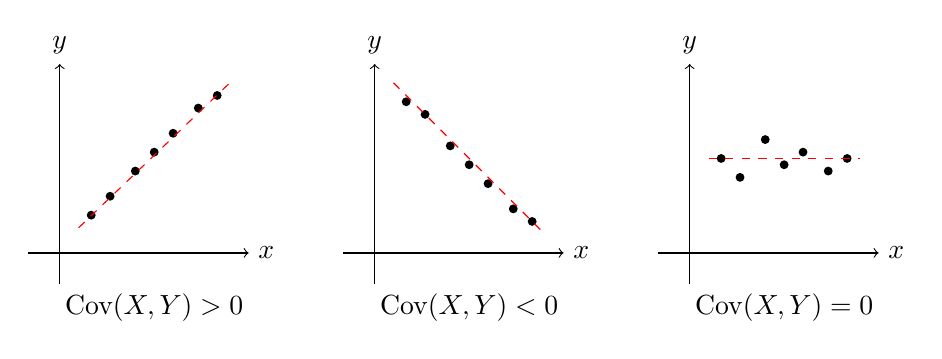
\begin{tikzpicture}[scale=0.8]
    % Positive covariance
    \begin{scope}[xshift=0cm]
        \draw[->] (-0.5,0) -- (3,0) node[right] {$x$};
        \draw[->] (0,-0.5) -- (0,3) node[above] {$y$};
        \foreach \x/\y in {0.5/0.6, 0.8/0.9, 1.2/1.3, 1.5/1.6, 1.8/1.9, 2.2/2.3, 2.5/2.5}
            \fill (\x,\y) circle (2pt);
        \draw[dashed, red] (0.3,0.4) -- (2.7,2.7);
        \node[below] at (1.5,-0.5) {Cov$(X,Y) > 0$};
    \end{scope}
    
    % Negative covariance
    \begin{scope}[xshift=5cm]
        \draw[->] (-0.5,0) -- (3,0) node[right] {$x$};
        \draw[->] (0,-0.5) -- (0,3) node[above] {$y$};
        \foreach \x/\y in {0.5/2.4, 0.8/2.2, 1.2/1.7, 1.5/1.4, 1.8/1.1, 2.2/0.7, 2.5/0.5}
            \fill (\x,\y) circle (2pt);
        \draw[dashed, red] (0.3,2.7) -- (2.7,0.3);
        \node[below] at (1.5,-0.5) {Cov$(X,Y) < 0$};
    \end{scope}
    
    % Zero covariance
    \begin{scope}[xshift=10cm]
        \draw[->] (-0.5,0) -- (3,0) node[right] {$x$};
        \draw[->] (0,-0.5) -- (0,3) node[above] {$y$};
        \foreach \x/\y in {0.5/1.5, 0.8/1.2, 1.2/1.8, 1.5/1.4, 1.8/1.6, 2.2/1.3, 2.5/1.5}
            \fill (\x,\y) circle (2pt);
        \draw[dashed, red] (0.3,1.5) -- (2.7,1.5);
        \node[below] at (1.5,-0.5) {Cov$(X,Y) = 0$};
    \end{scope}
\end{tikzpicture}
\end{center}
但是注意:
\begin{itemize}
    \item covariance 只捕捉 linear relationship, 即趋势是否呈直线,
不过不能捕捉 nonlinear relationship. 之后在学习 independence 的时候, 
我们会知道即便 covariance 为 0, \(X\) 和 \(Y\) 仍然可能是 dependent 的.
比如, 如果 \((X,Y)\) 的联合分布 as a graph 是个圆圈, 那么 covariance 
就是 0, 但显然这两个变量之间是有关系的.
\begin{center}
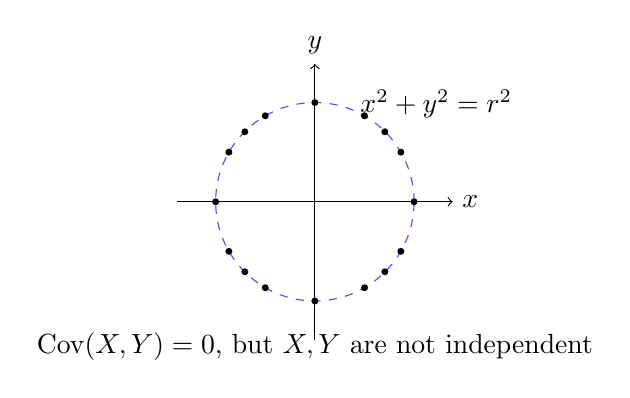
\begin{tikzpicture}[scale=0.7]
    \draw[->] (-2.5,0) -- (2.5,0) node[right] {$x$};
    \draw[->] (0,-2.5) -- (0,2.5) node[above] {$y$};
    \draw[dashed, blue!70] (0,0) circle (1.8);
    \foreach \x/\y in {
        1.8/0, 1.27/1.27, 0/1.8, -1.27/1.27,
        -1.8/0, -1.27/-1.27, 0/-1.8, 1.27/-1.27,
        1.56/0.9, 0.9/1.56, -0.9/1.56, -1.56/0.9,
        -1.56/-0.9, -0.9/-1.56, 0.9/-1.56, 1.56/-0.9
    }
        \fill (\x,\y) circle (1.8pt);
    \node[above right] at (0.65,1.35) {$x^2+y^2=r^2$};
    \node[below] at (0,-2.2) {Cov$(X,Y)=0$, but $X,Y$ are not independent};
\end{tikzpicture}
\end{center}

\item Covariance 的数值还包括了这两个 random variables 的 scale,
  因而还不能直接用来比较不同 random variables
  之间的 linear relationship 的强弱程度. 真正公平的 
  linear relationship 还需要 normalize by norms,
  把这个关系定位到 $[-1,1]$ 的区间上 即等下定义的 correlation.
\end{itemize}
 
\end{remark}


我们容易发现一件事情:
\begin{theorem}{covariance 是一个 a positive semi-definite symmetric bilinear form}
\begin{itemize}
\item covariance 是一个 \textbf{symmetric bilinear form }(并且 \textbf{translation-invariant}, 忽略 translation) 的 operator: 
    \[\text{Cov}(aX+b, cY+d) = ac \, \text{Cov}(X,Y) \]
    \[\text{Cov}(X,Y) = \text{Cov}(Y,X)\]
    \[\text{Cov}(X+Y, Z) = \text{Cov}(X, Z) + \text{Cov}(Y, Z)\]
    \item covariance 满足 positive definiteness: \(\text{Cov}(X,X) = \text{Var}(X) \geq 0\).
\end{itemize}
\end{theorem}
\begin{proof}
By def.
\end{proof}

而当我们把空间限定在 $L^2_0(\Omega, \mathcal{F}, \mathbb{P})$ 上时, 
\begin{theorem}{$L^2_0(\Omega, \mathcal{F}, \mathbb{P})$ 为一个 Hilbert space, with covariance as an inner product}
    $\big(L^2_0(\Omega, \mathcal{F}, \mathbb{P}), \langle \cdot, \cdot \rangle_{\text{Cov}} \big)$ 为一个 Hilbert space,
    即: covariance 在其上是一个 inner product (positive definite symmetric bilinear form).
\end{theorem}
\begin{proof}
很显然. 因为在 $L^2$ space 上, 一个 constant random variable 的
variance 是 0, 但是它并不是一个零函数; 而在 $L^2_0$ space 上, 
所有的 random variables 都是 zero-centered 的,
因而 constant random variable 就是零函数了. 
从而 covariance 在 $L^2_0$ space 上是 positive definite 的, 从而是 inner product.\\
\end{proof}


而在 $L^2_0(\Omega, \mathcal{F}, \mathbb{P})$ 上, 
两个 random variables \(X, Y\) 之间的夹角 \(\theta\) 的 cosine, 就是它们
真正的 linear relationship 的强弱程度, 因而我们把它叫做 correlation:
\begin{definition}{correlation}\label{def:correlation}
$$
\rho(X, Y)=\frac{\operatorname{Cov}(\mathrm{X}, \mathrm{Y})}{\sqrt{\operatorname{Var}(X)} \sqrt{\operatorname{Var}(Y)}}
$$
\end{definition}
显然, \[
\rho(X, Y) = \cos \theta
\]
where \(\theta\) 是 \(X, Y\) 之间的夹角.
And we have: \[
\text{Cov}(X,Y) =  \sigma_X \sigma_Y \rho(X,Y)
\]
从而有以下显然的结论: 
\begin{proposition}{properties of correlation}
    \begin{itemize}
    \item \(\rho(X,Y) \in [-1,1]\)
    \item 如果 \(\rho(X,Y) = 1\), 那么 \(Y = aX + b\) for some \(a > 0\) and \(b\); 如果
     \(\rho(X,Y) = -1\), 那么 \(Y = aX + b\) for some \(a < 0\) and \(b\).\
    \item By Cauchy-Schwarz inequality, \(|\text{Cov}(X,Y)| \leq \sigma_X \sigma_Y\).
\end{itemize}
\end{proposition}

做一个总结: 
\begin{center}
\renewcommand{\arraystretch}{1.25}
\setlength{\tabcolsep}{6pt}
\small
\begin{tabular}{|p{2.6cm}|p{5cm}|p{5cm}|}
\hline
& \textbf{$L^2$ space} & \textbf{$L_0^2$} \\
\hline
inner product $\langle X,Y\rangle$ & $\mathbb{E}[XY]$ & $\operatorname{Cov}(X,Y)$ (covariance) \\
\hline
norm $\|X\|$ & $\sqrt{\mathbb{E}[X^2]}$ & $\sqrt{\operatorname{Var}(X)}$ (standard deviation) \\
\hline
cosine similarity & $\frac{\mathbb{E}[XY]}{\sqrt{\mathbb{E}[X^2]} \sqrt{\mathbb{E}[Y^2]}}$ & $\frac{\operatorname{Cov}(X,Y)}{\sqrt{\operatorname{Var}(X)} \sqrt{\operatorname{Var}(Y)}}$ (correlation) \\
\hline
\end{tabular}
\end{center}
\textbf{求两个 random variables 之间的 correlation, 
就是把它们都 center 到 zero-centered 的位置 (即投影到 $L_0^2$ space 上),
然后计算它们在 $L_0^2$ space 上的 cosine similarity.}\\







此时我们看到 decomposition of variance: 
\begin{proposition}{两个 random variables 之和的 variance}
两个 random variables 的和的 variance 可分解成 variances 和 covariance:  
 \[\text{Var}(X+Y) = \text{Var}(X) + \text{Var}(Y) + 2\text{Cov}(X,Y)\]
\end{proposition}
\begin{proof}
 $$
\operatorname{Var}(X+Y)=\mathbb{E}\left[(X+Y)^2\right]-(\mathbb{E}[X+Y])^2=\mathbb{E}\left[X^2\right]-(\mathbb{E}[X])^2+\mathbb{E}\left[Y^2\right]-(\mathbb{E}[Y])^2+2(\mathbb{E}[X Y]-\mathbb{E}[X] \mathbb{E}[Y])
$$
\end{proof}
\begin{remark}

它其实这就是标准的 inner product space 上的向量平方公式:
$$
\|X+Y\|_{L_0^2}^2=\|X\|_{L_0^2}^2+\|Y\|_{L_0^2}^2+2\langle X, Y\rangle_{L_0^2}
$$
\end{remark}






\section{discrete random variables}
Recall: discrete random variable 是指其 range a.s. 是 countable 的 random variable.
(存在一个 countable set \(S \subseteq \mathbb{R}\) 
     使得 \(\bP(X \in S) = 1\))

discrete RV 的 probability mass unction (pmf):
        \[
        p_X(x) := \bP(X = x), \quad \forall x \in \mathbb{R}
        \]
就是 \(X\) 的 distribution \(P^X\) 对于 counting measure of range \(S\)
的 Radon-Nikodym derivative:
     \[
     p_X = \frac{d\bP^X}{d\mu_{\text{S}}}
     \]

因为假设 \(X\) 的 range 是 \(S = \{x_1, x_2, \ldots\}\), 
    那么对于任意 Borel set \(B\),
    \[
    \bP^X(B) = \sum_{x_i \in B} \bP(X = x_i) = \sum_{x_i \in B\cap S} p_X(x_i) = 
    \int_A p_X(x) \;d\mu_{\text{S}}(x)
     \]     



下面我们给出一些经典的 discrete random variable 的例子, 以及它们的 pmf 和 cdf.

\subsection{Bernoulli distribution and Binomial distribution}
\begin{example}{(\textbf{Bernoulli distribution})}
    
    令 \(\Omega:= \{\omega_1, \omega_2\}\), \(\cF := 2^{\Omega}\).\\
    令 \(\bP(\{\omega_1\}) = p\), \(\bP(\{\omega_2\}) = 1-p\) 来表示这两个 singular 事件的概率.\\
    令 \(X(\omega_1) = 1\), \(X(\omega_2) = 0\) 分别表示 success 和 failure.\\
    那么显然可以计算:
    \[
    \bP(X=0) = \bP(\{\omega_2\}) = 1-p, \quad \bP(X=1) = \bP(\{\omega_1\}) = p
    \]
    我们称 \((\Omega, \mathcal{F}, \bP)\) 为一个 Bernoulli probability space 
    (它 model 了一个 Bernoulli trial, 即一个 random experiment with two possible outcomes: success 和 failure)\\
    称 \(X: \Omega \to \{0,1\}\) 这个 random variable 为一个 \textbf{Bernoulli random variable},
    并称 \(X\) 的 distribution \(P^X\) 为一个 \textbf{Bernoulli distribution}, 写作
    \[
    X \sim \text{Ber}(p)
    \]
    这是最简单的 random variable 和 distribution 了. 它 model 的是: 
    比如我们 toss 一枚 biased coin, 
    以 \(p\) 的概率得到 heads (success), 
    以 \(1-p\) 的概率得到 tails (failure).\\
\end{example}

\begin{proposition}
    如果 \(X \sim \text{Ber}(p)\), 
    那么 \(\bE[X] = p\), \(\text{Var}(X) = p(1-p)\).
\end{proposition}
显然.

\begin{example}{(\textbf{Binomial distribution})}

我们 independently repeat \(n\) 次 Bernoulli trial, 
每次 trial 的 success probability 都是 \(p\).\\
考虑:
\[
S := X_1 + X_2 + \cdots + X_n
\] 为 success 的总次数. 那么 \(S\) 是一个 discrete random variable 
\( S: \Omega^n \to \mathbb{Z}_{\geq 0}  \)
容易计算出 \(S\) 的 pmf:
\[
p_S(k) = \bP(S = k) = \binom{n}{k} p^k (1-p)^{n-k}, \quad k = 0,1,\ldots,n
\]
我们称 \(S\) 的 distribution \(P^S\) 为一个 \textbf{Binomial distribution}, 写作
\[
S \sim \text{Bin}(n,p)
\]
它 model 的是: 比如我们 toss 一枚 biased coin \(n\) 次,
得到 heads 的总次数.\\
\end{example}
\begin{proposition}
    如果 \(S \sim \text{Bin}(n,p)\), 那么 \(\bE[S] = np\), \(\text{Var}(S) = np(1-p)\).
\end{proposition}
\begin{proof}
    \[
    \bE[X] = \sum_{k=1}^n k \cdot \bP(X = k) = 
    \sum_{k=1}^n k \cdot \binom{n}{k} p^k (1-p)^{n-k} =
    p(1-p)^{n-1} \sum_{k=1}^n k \cdot \binom{n}{k} (\frac{p}{1-p})^{k-1}
    \]
    由于 \[
    (1+t)^n = \sum_{k=0}^{n} \binom{n}{k} t^k \implies n(1+t)^{n-1} = \sum_{k=1}^n k \cdot \binom{n}{k} t^{k-1}
    \]
    可以得到 \[
    \bE[X] = p(1-p)^{n-1} \cdot n(1+\frac{p}{1-p})^{n-1} = np
    \]
    然后计算得
    \(
    \text{Var}(X) = np(1-p)
    \). 但是这是比较麻烦的方法. 
    也可以利用 \(X = \sum_{i=1}^n X_i\), 
    其中 \(X_i \sim \text{Ber}(p)\) i.i.d 这个事实来计算, 那么直接通过
    线性叠加 Bernoulli random variable 的 expectation 和 variance 就可以了.
\end{proof}

\subsection{Geometric distribution and Negative Binomial distribution}
\begin{example}{(\textbf{Geometric distribution})}

我们 perform independent Bernoulli trial, 每次 trial 的 success probability 都是 \(p\).\\
考虑 random variable \(T\) 表示第一次 success 发生的 trial number. (也就是等于: 我们一直 trial, 直到第一次 success 发生, 那么这个 trial 的 number 就是 \(T\)).\\
那么 \(T\) 是一个 discrete random variable \(T: \Omega^\infty \to \mathbb{Z}_{\geq 1}\).\\
容易计算出 \(T\) 的 pmf:
\[
p_T(k) = \bP(T = k) = (1-p)^{k-1} p, \quad k = 1,2,\ldots
\]
我们称 \(T\) 的 distribution \(P^T\) 为一个 \textbf{Geometric distribution}, 写作
\[
T \sim \text{Geom}(p)
\]
它 model 的是: 比如我们 toss 一枚 biased coin, 
第一次得到 heads 的 trial number.\\
\end{example}
\begin{proposition}
    如果 \(X \sim \text{Geom}(p)\), 那么 \(\bE[X] = 1/p\),
     \(\text{Var}(X) = (1-p)/p^2\).
\end{proposition}
\begin{proof}
    \[
    \bE[X] = \sum_{k=1}^\infty k(1-p)^{k-1}p = p\sum_{k=1}^\infty k(1-p)^{k-1} = 
    p \big( -\frac{d}{d(1-p)} \sum_{k=0}^\infty (1-p)^k \big) = 
    -p -\frac{d}{dp} \frac{1}{1-(1-p)}  = \frac{1}{p}
    \]
    similarly, 可以计算得\[
    \bE[X^2] =\frac{2-p}{p^2}
    \]
    因而 \[
    \text{Var}[X] = \bE[X^2] - (\bE[X])^2 = \frac{1-p}{p^2}
    \]
\end{proof}


\begin{example}{(\textbf{Negative Binomial distribution})}

这是 Geometric distribution 的 generalization (但不完全一样).\\
我们 perform independent Bernoulli trial, 
每次 trial 的 success probability 都是 \(p\). (即 independent and identically distributed)\\
令 random variable \(T_r\) 表示第 \(r\) 次 success 发生之前
的 failures 的数量.
 (也就是等于: 我们一直 trial, 直到第
\(r\) 次 success 发生, 那么这个 trial 的 number 就是 \(T_r + r\), 
因为 \(T_r\) 是 failures 的数量, 还要加上 \(r-1\) 个 success.
).\\
那么 \(T_r\) 是一个 discrete random variable 
\(T_r: \Omega^\infty \to \mathbb{Z}_{\geq 0}\).\\
容易计算出 \(T_r\) 的 pmf:
\[
p_{T_r}(k) = \bP(T_r = k) = 
\binom{k+r-1}{k}  (1-p)^{k} p^r, \quad k = 0, 1, 2, \ldots
\]
这是因为:最后一次 success 的位置是固定的. 我们要在前 \(k+r-1\) 次 trial 
中选择 \(k\) 次作为 failures.\\
我们称 \(T_r\) 的 distribution \(P^{T_r}\) 为一个 \textbf{Negative Binomial distribution}, 写作
\[
T_r \sim \text{NB}(r,p)
\]  
它 model 的是: 比如我们 toss 一枚 biased coin,
得到第 \(r\) 个 heads 之前会经历的 failures 的数量.\\
\end{example}


\subsection{Poisson distribution}
\begin{example}{(\textbf{Poisson distribution})}
考虑这一 pmf:
\[
\bP(X=k) = e^{-\lambda} \frac{\lambda^k}{k!}, \quad k = 0, 1, 2, \ldots
\]
我们称 \(X\) 的 distribution \(P^X\) 为一个 \textbf{Poisson distribution}, 写作
\[
X \sim \text{Poi}(\lambda), \quad \lambda > 0
\]
以 \(\lambda=3\) 为例画出 pmf 示意图:
\begin{center}
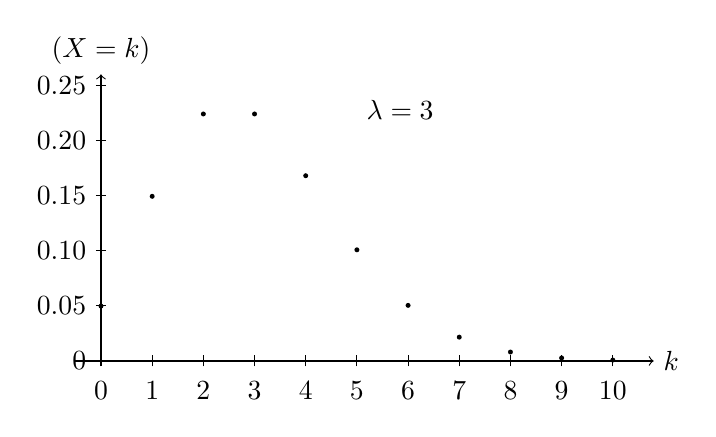
\begin{tikzpicture}[x=0.65cm,y=14cm]
    \draw[->] (-0.5,0) -- (10.8,0) node[right] {$k$};
    \draw[->] (0,0) -- (0,0.26) node[above] {$\bP(X=k)$};
    
    % y轴刻度标注
    \foreach \y in {0, 0.05, 0.10, 0.15, 0.20, 0.25} {
        \draw (-0.1,\y) -- (0.1,\y);
        \node[left] at (-0.1,\y) {\y};
    }
    
    % x轴刻度标注
    \foreach \x in {0, 1, 2, 3, 4, 5, 6, 7, 8, 9, 10} {
        \draw (\x,-0.005) -- (\x,0.005);
        \node[below] at (\x,-0.01) {\x};
    }
    
    % \lambda=3 时, k=0..10 的 pmf 数值（避免 pgfmath 阶乘/幂运算溢出）
    \foreach \kv/\pv in {
        0/0.04979,
        1/0.14936,
        2/0.22404,
        3/0.22404,
        4/0.16803,
        5/0.10082,
        6/0.05041,
        7/0.02160,
        8/0.00810,
        9/0.00270,
        10/0.00081
    } {
        \fill (\kv,\pv) circle (0.9pt);
    }
    \node[above right] at (5,0.21) {$\lambda=3$};
\end{tikzpicture}
\end{center}
\begin{remark}
当 \(n\to\infty\) 时, 
\(\text{Bin}(n, \lambda/n)\) 的 distribution 
趋近于 \(\text{Poi}(\lambda)\).\\
考虑 $X \sim B\left(n, \frac{\lambda}{n}\right)$, 对于固定的 $k$:
$$
\bP(X=k)=\binom{n}{k}\left(\frac{\lambda}{n}\right)^k\left(1-\frac{\lambda}{n}\right)^{n-k}
$$
展开组合数 $\binom{n}{k}$:
$$
\bP(X=k)=\frac{n(n-1) \ldots(n-k+1)}{k!} \cdot \frac{\lambda^k}{n^k} \cdot\left(1-\frac{\lambda}{n}\right)^n \cdot\left(1-\frac{\lambda}{n}\right)^{-k}
$$
重组项:
$$
\bP(X=k)=\frac{\lambda^k}{k!} \cdot \underbrace{\frac{n(n-1) \ldots(n-k+1)}{n^k}}_{(1)} \cdot \underbrace{\left(1-\frac{\lambda}{n}\right)^n}_{(2)} \cdot \underbrace{\left(1-\frac{\lambda}{n}\right)^{-k}}_{(3)}
$$
其中, (1) 的 limit 是 1, 
(2) 的 limit 是 $e^{-\lambda}$, (3) 的 limit 是 1, 因而 
\[
\lim_{n\to\infty} \mathbb{P}(X=k)= e^{-\lambda} \frac{\lambda^k}{k!}
\]
这个极限行为的意义是:
\begin{itemize}
    \item \(\lambda \) 表示: 在一个固定时间/空间窗口内, 一个事件出现的平均次数的观测.
    \item 我们把这段时间间分成 \(n\) 个小窗口, 将这个观测作为先验知识用来 model 这类事件实现的平均概率, 那么
     每个小窗口内事件出现的概率是 \(p = \lambda/n\).  
    \item 每个 \(\text{Bin}(n,\lambda / n)\) 都表示: 在时间细分成
     \(n\) 个小窗口的情况下, 这个事件出现的次数的分布. (注意不是在时间上的分布, 而是在次数上的分布)
    \item 当 \(n\to\infty\) 时, 其意义: 基于连续时间的估计, 
    这个事件在原固定事件窗口内出现的次数的分布. 这就是 
    \(\text{Poi}(\lambda)\) 的意义.
\end{itemize}
因而 Poisson distribution 的意义本质上是: 
\textbf{
给定对一个事件在固定窗口下出现的平均次数的观测(估计), 
那么这个事件在这个窗口内出现 \(n\) 次 
(\(n = 0,1,2,\cdots  \))的概率是多少?}\\
所以 Poisson 分布, 即是\textbf{根据一个事件在给定 windows 内发生次数的 expectation, 来估计这个事件在该 windows 内发生次数的分布的标准方法.}  \\
\end{remark}

\begin{remark}

Further remark: Poisson distribution 的用途.
\begin{itemize}
    \item 它是 model "大量级的小概率事件" 的通用模型.\\ 
    即一段时间内, 一件事情的发生的概率非常小 (\(p \ll 1\)), 
    但是有很多机会发生 (\(n \gg 1\)). 比如放射性衰变.
    \item 现实世界中, 对于一些事情, 我们想要 model 其在一段时间内发生的总次数 (\(n\)) 和单次成功率 (\(p\)) 
    是很困难的. 比如统计今天路过百货大楼的总人数 (\(n\)), 以及每个人路过百货大楼时走进去的概率 (\(p\)). 但是我们
    很容易可以知道: \(\lambda = np\) 的观测. 即: 每天平均有多少人走进百货大楼. 那么我们就可以用 Poisson distribution 来 model 这件事情在一天内发生的次数的分布.\\
\end{itemize}
\end{remark}
\end{example}

\begin{proposition}
    如果 \(X \sim \text{Poi}(\lambda)\), 那么 \(\bE[X] = \lambda\), \(\text{Var}(X) = \lambda\).
\end{proposition}
\begin{proof}
recall \(e^x\) 的 taylor expansion: \[
e^x = \sum_{k=0}^\infty \frac{x^k}{k!}
\]
因而
    \[
    \bE[X] = \sum_{k=0}^\infty k e^{-\lambda} \frac{\lambda^k}{k!} = 
    e^{-\lambda} \lambda \sum_{k=1}^\infty \frac{\lambda^{k-1}}{(k-1)!} =
    e^{-\lambda} \lambda e^{\lambda} = \lambda
    \]
similarly, 可以计算得 \[
\bE[X^2] = \lambda^2 + \lambda
\]
因此, \[
\text{Var}(X) = \bE[X^2] - (\bE[X])^2 = \lambda
\]
\end{proof}


\subsubsection{Poisson distribution 的 additivity}
\begin{theorem}{additivity of Poisson distribution}
    如果 \(X \sim \text{Poi}(\lambda_1)\), \(Y \sim \text{Poi}(\lambda_2)\) are independent, 那么
    \[
    X + Y \sim \text{Poi}(\lambda_1 + \lambda_2)
    \]
\end{theorem}
\begin{remark}
这个事实通过简单的计算即可得到. 

但是值得一提的是, 我们之后会证明一个结论: 两个 independent 的 random variable 
的 sum 的 distribution 是它们 convolution 的 distribution.

而 Poisson distribution 的 convolution 仍然是 Poisson distribution, 
并且是 linear 的. 这就是 additivity of Poisson distribution 的本质原因.
\end{remark}



\section{continuous random variables}
recall: 总而言之, continuous random variable 是指其 distribution \(\bP^X\)
对于 Lebesgue measure \(m\) 是 absolutely continuous 的 random variable, 
等价于存在一个 pdf \(f_X\) 使得\[
F_X(x) = \int_{-\infty}^x f_X(y) dy 
\] 对于任意 \(x\) 都成立.

而由 \( \bE[X]= \int_{\Omega} X d\bP = \int_{\mathbb{R}} x d\bP^X = \int_{\mathbb{R}} x f_X(x) dx \) 可得 
\[
\bE[X] = \int_{-\infty}^{+\infty} x f_X(x) dx, \quad \text{Var}(X) = \int_{-\infty}^{+\infty} (x-\bE[X])^2 f_X(x) dx
\]

这里还有一个额外的结论:
\begin{proposition}
     对于任意的 measurable function \(g: \bR \to \bR\), 都有
\[
\bE[g(X)] = \int_{-\infty}^{+\infty} g(x) f_X(x) dx
\]
\end{proposition}
\begin{proof}
\begin{align*}
\bE[g(X)] &= \int_{\Omega} g(X(w))\, d\bP(w) \\
&=  \int_{\Omega} g\circ X \, d\bP \\
&= \int_{\bR} g \, d\bP^X \\
&= \int_{-\infty}^{+\infty} g(x) f_X(x) \, dx
\end{align*}
\end{proof}

下面我们介绍一些常见的 continuous random variables, 以及它们的 pdf, cdf, expectation 和 variance.

\subsection{uniform distribution: 最简单的 continuous RV}
\begin{definition}{uniform distribution}
如果 \(f_X(x) = \frac{1}{b-a}\) on \((a,b)\) and \(0\) elsewhere,
那么我们称 \(X\) 的 distribution \(P^X\) 为一个 
\textbf{uniform distribution}, 写作
\[
X \sim U([a,b])
\]
\end{definition}

对于 uniform distribution, 很容易计算得:
\[
F_X(x) = \frac{x-b}{b-a}, \quad \bE[X] = \frac{a+b}{2}, \quad 
\text{Var}(X) = \frac{(b-a)^2}{12}
\]
\begin{example}{(uniform distribution 的 pdf 和 cdf)}
    
考虑 $X \sim U([a,b])$, 其 pdf 和 cdf 的图像如下:
\begin{center}
\begin{minipage}{0.48\textwidth}
    \centering
    \begin{tikzpicture}[x=1cm, y=2cm]
        % PDF subplot
        \draw[->] (-0.5,0) -- (5,0) node[right] {$x$};
        \draw[->] (0,-0.3) -- (0,1.2) node[above] {$f_X(x)$};
        
        % Line at x=a, x=b
        \draw[dashed, gray] (1,-0.2) -- (1,0);
        \draw[dashed, gray] (4,-0.2) -- (4,0);
        \node[below] at (1,-0.25) {$a$};
        \node[below] at (4,-0.25) {$b$};
        
        % PDF function
        \draw[line width=1.5pt] (1,0.75) -- (4,0.75);
        \draw[line width=1.5pt] (0.5,0) -- (1,0);
        \draw[line width=1.5pt] (4,0) -- (4.5,0);
        
        % Vertical lines at endpoints
        \draw[line width=1pt, dashed] (1,0) -- (1,0.75);
        \draw[line width=1pt, dashed] (4,0) -- (4,0.75);
        
        \node at (2.5,1) {$\frac{1}{b-a}$};
        \node at (2.5,-0.8) {pdf: $f_X(x) = \frac{1}{b-a}$};
        
    \end{tikzpicture}
\end{minipage}
\hfill
\begin{minipage}{0.48\textwidth}
    \centering
    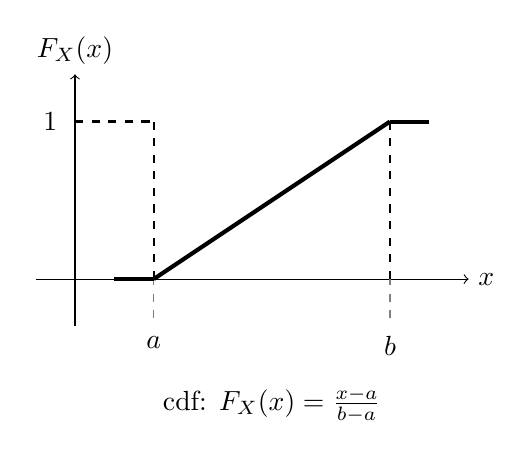
\begin{tikzpicture}[x=1cm, y=2cm]
        % CDF subplot
        \draw[->] (-0.5,0) -- (5,0) node[right] {$x$};
        \draw[->] (0,-0.3) -- (0,1.3) node[above] {$F_X(x)$};
        
        % Line at x=a, x=b
        \draw[dashed, gray] (1,-0.25) -- (1,0);
        \draw[dashed, gray] (4,-0.25) -- (4,0);
        \node[below] at (1,-0.3) {$a$};
        \node[below] at (4,-0.3) {$b$};
        
        % CDF function: flat at 0, then linear, then flat at 1
        \draw[line width=1.5pt] (0.5,0) -- (1,0);
        \draw[line width=1.5pt] (1,0) -- (4,1);
        \draw[line width=1.5pt] (4,1) -- (4.5,1);
        
        % Vertical lines at endpoints
        \draw[line width=0.8pt, dashed] (1,0) -- (1,1);
        \draw[line width=0.8pt, dashed] (4,0) -- (4,1);
        \draw[line width=0.8pt, dashed] (0,1) -- (1,1);
        
        \node[left] at (-0.1,1) {$1$};
        \node at (2.5,-0.8) {cdf: $F_X(x) = \frac{x-a}{b-a}$};
        
    \end{tikzpicture}
\end{minipage}
\end{center}

\end{example}


\subsection{exponential distribution: geometric distribution 的 continuous version}
Exponential random variable model 的是一盏灯的 remaining lifetime. 
它 assume: 任意时间, 这盏灯有一个 constant 的磨损速率.

假设它的磨损速率是 \(\lambda = \lambda_X(t)\) for all \(t\), 
那么在任意时间 \(t\) 上:
\[
\lambda_X(t) = \lim_{h\to 0^+} \frac{P(X \in (t, t+h])}{h} 
= \lim_{h\to0^+}\frac{\bP(t \leq X \leq t+h)}{h}  \cdot \frac{1}{\bP(X > t)}
= \frac{f_X(t)}{1 - F_X(t)}
\]

即 ODE: 
\[
\lambda = \frac{F_X'(t)}{1 - F_X(t)}
\]
with initial condition \(F_X(0) = 0\).

我们知道这个 ODE 的 solution 是: \[
F_X(t) = \begin{cases}
    1 - e^{-\lambda t}, \quad t > 0\\
    0, \quad t \leq 0
\end{cases},
\quad 
f_X(t) = \begin{cases}
    \lambda e^{-\lambda t}, \quad t > 0\\
    0, \quad t \leq 0 
\end{cases}
\]

\begin{definition}{exponential distribution}
我们称 $X$ 为一个 \textbf{exponential random variable} with parameter $\lambda$,
如果它的 pdf is given by: \[
f(x) = \begin{cases}
    \lambda e^{-\lambda x}, \quad x > 0\\
    0, \quad x \leq 0
\end{cases}
\]
写作\[  
X \sim \text{Exp}(\lambda)
\]
\end{definition}
刚才已经计算出, exponential random variable 的
distribution 为\[
F_X(x) = \begin{cases}
    \int _{-\infty}^x f(t) \; dt = \lambda \int_0 ^x e^{-\lambda t} \; dt = 1 - e^{-\lambda x}, \quad x> 0\\
    0,\quad x<0
\end{cases}
\]
容易验证, $F_X(x) =0$ when $x \to -\infty$, 以及 $F_X(x) \to 1$ when $x \to \infty$

计算其 expectation:
\begin{align}
\mathbb{E}[X^n] &= \lambda \int_0^\infty x^n e^{-\lambda x } \; dx  \\
&= - \int_0 ^\infty  x^n(e^{-\lambda x})' \; dx \\
&=  0 + \int_0 ^\infty n x^{n-1} e^{-\lambda x} \; dx \\
&= \frac{n}{\lambda} \mathbb{E}(X^{n-1})
\end{align}
并 notice: $\mathbb{E}[X^0] = \mathbb{E}[1] = 1$. 
因而 recursively get: \[
\mathbb{E}[X^n] = \frac{n!}{\lambda^n}
\]
即: 
\(\mathbb{E}[X] = \frac{1}{\lambda}, \mathbb{E}[X^2] = \frac{2}{\lambda^2}, \cdots  \)
从而: \[
Var[X] = \frac{2}{\lambda^2} - \frac{1}{\lambda^2} = \frac{1}{\lambda^2}
\]

\begin{center}
\begin{minipage}{0.48\textwidth}
    \centering
    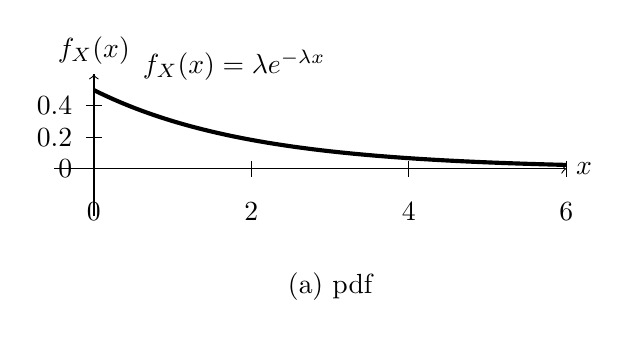
\begin{tikzpicture}[x=1cm, y=2cm]
        % PDF subplot
        \draw[->] (-0.5,0) -- (6,0) node[right] {$x$};
        \draw[->] (0,-0.3) -- (0,0.6) node[above] {$f_X(x)$};
        
        % x轴刻度
        \foreach \x in {0, 2, 4, 6} {
            \draw (\x,-0.05) -- (\x,0.05);
            \node[below] at (\x,-0.15) {\x};
        }
        
        % y轴刻度
        \foreach \y in {0, 0.2, 0.4} {
            \draw (-0.1,\y) -- (0.1,\y);
            \node[left] at (-0.15,\y) {\y};
        }
        
        % PDF function: lambda * e^(-lambda*x)
        \draw[line width=1.5pt, domain=0:6, samples=100] plot (\x, {0.5*exp(-0.5*\x)});
        
        % y轴
        \draw[line width=0.8pt] (0,-0.3) -- (0,0.6);
        
        \node[above right] at (0.5,0.5) {$f_X(x) = \lambda e^{-\lambda x}$};
        \node[below] at (3,-0.6) {(a) pdf};
        
    \end{tikzpicture}
\end{minipage}
\hfill
\begin{minipage}{0.48\textwidth}
    \centering
    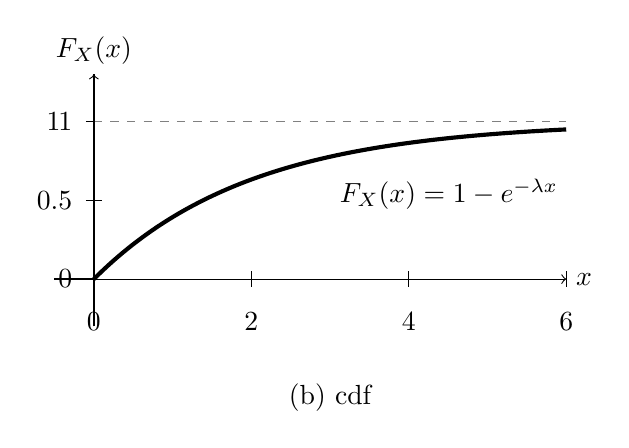
\begin{tikzpicture}[x=1cm, y=2cm]
        % CDF subplot
        \draw[->] (-0.5,0) -- (6,0) node[right] {$x$};
        \draw[->] (0,-0.3) -- (0,1.3) node[above] {$F_X(x)$};
        
        % x轴刻度
        \foreach \x in {0, 2, 4, 6} {
            \draw (\x,-0.05) -- (\x,0.05);
            \node[below] at (\x,-0.15) {\x};
        }
        
        % y轴刻度
        \foreach \y in {0, 0.5, 1} {
            \draw (-0.1,\y) -- (0.1,\y);
            \node[left] at (-0.15,\y) {\y};
        }
        
        % CDF function: 1 - e^(-lambda*x) for x >= 0
        \draw[line width=0.8pt] (-0.5,0) -- (0,0);
        \draw[line width=1.5pt, domain=0:6, samples=100] plot (\x, {1-exp(-0.5*\x)});
        
        % 水平虚线在y=1处
        \draw[dashed, gray] (0,1) -- (6,1);
        \node[left] at (-0.3,1) {$1$};
        
        % y轴
        \draw[line width=0.8pt] (0,-0.3) -- (0,1.3);
        
        \node[below right] at (3,0.7) {$F_X(x) = 1 - e^{-\lambda x}$};
        \node[below] at (3,-0.6) {(b) cdf};
        
    \end{tikzpicture}
\end{minipage}
\end{center}


\begin{remark}
exponential 随机变量是 geometric 随机变量的 continuous analogue.
因为 geometric random variable 是假设一个事件在 
每个时间点以 constant 的概率发生,
用来 model 它第一次发生的时间;

而 exponential random variable 其实也是, 只是 on a continuous
 time scale: 
 它假设的 constant 损坏率其实 implies:
\textbf{在任意时间, 如果灯还没坏, 那么灯此刻坏掉的概率是 constant 的.} 
\begin{theorem}{memoryless property of exponential distribution}
任意 continuous RV, \[
 \bP(X > b+ t \mid X > b) = \bP(X>t) \iff X \text{ is an exponential random variable}
    \]
\end{theorem}
\begin{proof}
简单而言
\begin{align}
     &   P(X > b+ t \mid X > b) = P(X>t) \\
   \Longleftrightarrow  & P(X > b+t) = P(X > t) P(X>b) \\
    \Longleftrightarrow  & X \text{ exponential}
\end{align}
\end{proof}
因而对于 geometric RV 的 pmf, 当我们把时间间隔 (discrete time interval) 变得越来越小,
这一行为的极限就变为了 exponential RV 的 pdf. 

这是一个很自然的 limit behavior, 此处不验证了.
\end{remark}

\begin{example}
假设我们有一个 storage battery, 它的 lifetime 是 exponentially distributed 的, 并且 average 为 10 hours. Suppose 我们想要 use this battery for 5 hours for.

计算: probability of finishing the task, if:\\
(a) 使用一个 new battery\\
(b) 使用一个已经用过 2 hours 的 battery\\
\begin{solution}
    \[
    \mathbb{E}[X] = 10 = \frac{1}{\lambda} \implies \lambda = \frac{1}{10}
    \]
如果我们使用一个 new battery, 则 want: $P(X>5) = 1 - P(X<5) = 1- F_X(5) = e^{-\frac{1}{2}}$
如果我们使用一个用过 2 hours 的 battery, 则 want: \[
P(X> 5+2 \mid X > 2) = \frac{e^{-(5+2)\lambda}}{e^{-2\lambda }} = e^{-5\lambda} = = e^{-\frac{1}{2}}
\]
Notice:  \[
P(X>5) = P(X> 5+2 \mid X > 2)
\]
\end{solution} 

\end{example}





\subsection{Gamma distribution: negative binomial distribution 的 continuous version}
recall Gamma 函数:
\[
    \Gamma(\alpha) = \int_0^\infty x^{\alpha - 1} e^{-x}\; dx
\]
这个函数有一个重要的性质: \[
\Gamma(\alpha + 1) = \alpha \Gamma(\alpha)  
\]
因而对于 \(n\in \mathbb{N}\), 我们有: \[
\Gamma(n) = (n-1)!
\]
Gamma 函数就是 factorial 函数的 continuous generalization.

\begin{definition}{$\Gamma$-distribution}
如果 continuous random variable $X$ 的 pdf 是: 
$$
f_X(x)= \begin{cases}
\displaystyle \frac{\lambda^\alpha}{\Gamma(\alpha)} x^{\alpha-1} e^{-\lambda x}, & x>0, \\ 
0, & x \leq 0 
\end{cases}
$$
那么我们称 $X$ 服从 \textbf{$\Gamma$ distribution}, 写作\[
X \sim \Gamma(\alpha, \lambda)
\]
其中 $\alpha > 0$ 称为 shape parameter, $\lambda > 0$ 称为 rate parameter.
\end{definition}

\(\Gamma\) distribution 的 cdf 这样求: for \(a \geq 0\),
\begin{align*}
    F_X(a) = \int_{-\infty}^a f_X(x) \; dx &= \int_0^a \frac{\lambda^\alpha}{\Gamma(\alpha)} x^{\alpha -1} e^{-\lambda x} \; dx \\
    &= \frac{1}{\Gamma(\alpha)} \int_0^{\lambda a} t^{\alpha -1} e^{-t} \; dt
\end{align*}
and for \(a < 0\), \(F_X(a) = 0\).


Expectation:  
\begin{align*}
    \mathbb{E}[X] &= \frac{1}{\Gamma(\alpha)} \int_0^\infty (\lambda x )^{\alpha -1} \lambda  e^{-\lambda x} \; dx\\
    &=  \frac{1}{\lambda \Gamma(\alpha)}  \int_0^\infty x^\alpha e^{-x} \; dx \\
    &= \frac{\Gamma(\alpha + 1)}{\lambda \Gamma(\alpha)} = \frac{\alpha}{\lambda}
\end{align*}
(since $\Gamma(\alpha + 1) = \alpha \Gamma(\alpha)$.)
同理我们可以计算得: \(
\mathbb{E}[X^2] = \frac{\alpha(\alpha+1)}{\lambda^2}
\)
从而 \[
\text{Var}[X] = \mathbb{E}[X^2] - (\mathbb{E}[X])^2 = \frac{\alpha(\alpha+1)}{\lambda^2} - \frac{\alpha^2}{\lambda^2} = \frac{\alpha}{\lambda^2}
\] 

容易发现: 当 \(\alpha = 1\) 时, \(\Gamma\) distribution 就退化成了 exponential distribution.
\[
\Gamma(1,\lambda) = \text{Exp}(\lambda)  
\]
而当 \(\alpha\) 是一个正整数 \(n\) 时, \(\Gamma\) distribution 实际就是 \(n\) 个 
independent exponential distribution 的 sum: 
\begin{proposition}{Gamma distribution 即是 independent exponential distribution 的 sum}
Let \(X_1, X_2, \cdots, X_n \sim \text{Exp}(\lambda)\) be i.i.d., 则 
\[
\Gamma(n,\lambda) = \sum_{i=1}^n X_i
\]

\end{proposition}
\begin{proof}
    证明这一结论除了硬算之外, 更快的方法是通过 moment generating function. 
    //TODO
\end{proof}


    \begin{remark}
        Gamma distribution 即多个 i.i.d. exponential distribution 的 sum; 而我们知道 
        exponential distribution 是 geometric distribution 的 continuous analogue; 
        因而 \textbf{Gamma distribution 也是 negative binomial distribution 的 continuous analogue.}

        考虑固定 rate parameter $\lambda = 1$，不同 shape parameter $\alpha$ 的 Gamma distribution：

        \begin{center}
        \begin{tabular}{cc}
            \begin{minipage}{0.48\textwidth}
                \centering
                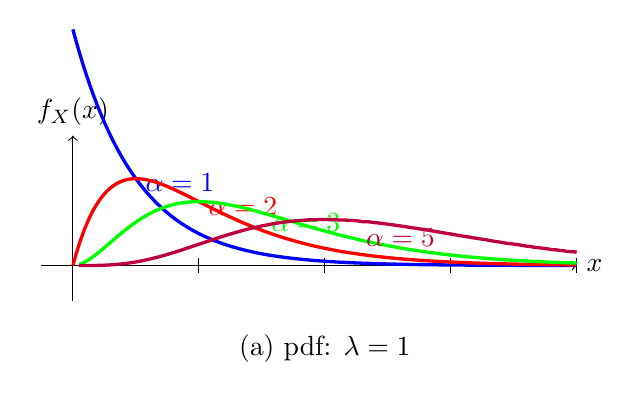
\begin{tikzpicture}[x=0.8cm, y=3cm]
                    % PDF subplot
                    \draw[->] (-0.5,0) -- (8,0) node[right] {$x$};
                    \draw[->] (0,-0.15) -- (0,0.55) node[above] {$f_X(x)$};
                    
                    % x轴刻度
                    \foreach \x in {0, 2, 4, 6, 8} {
                        \draw (\x,-0.03) -- (\x,0.03);
                    }
                    
                    % Gamma(1,1) = Exp(1)
                    \draw[line width=1.2pt, domain=0:8, samples=150, blue] plot (\x, {exp(-\x)});
                    \node[blue, right] at (1,0.35) {$\alpha=1$};
                    
                    % Gamma(2,1)
                    \draw[line width=1.2pt, domain=0:8, samples=150, red] plot (\x, {\x*exp(-\x)});
                    \node[red, right] at (2,0.25) {$\alpha=2$};
                    
                    % Gamma(3,1)
                    \draw[line width=1.2pt, domain=0.1:8, samples=150, green] plot (\x, {0.5*\x*\x*exp(-\x)});
                    \node[green, right] at (3,0.18) {$\alpha=3$};
                    
                    % Gamma(5,1)
                    \draw[line width=1.2pt, domain=0.1:8, samples=150, purple] plot (\x, {(1/24)*\x*\x*\x*\x*exp(-\x)});
                    \node[purple, right] at (4.5,0.12) {$\alpha=5$};
                    
                    \node at (4,-0.35) {(a) pdf: $\lambda=1$};
                \end{tikzpicture}
            \end{minipage} &
            \begin{minipage}{0.48\textwidth}
                \centering
                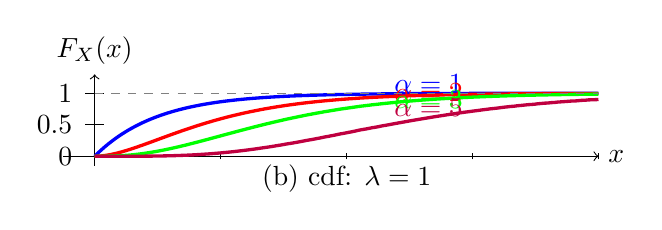
\begin{tikzpicture}[x=0.8cm, y=0.8cm]
                    % CDF subplot
                    \draw[->] (-0.5,0) -- (8,0) node[right] {$x$};
                    \draw[->] (0,-0.15) -- (0,1.3) node[above] {$F_X(x)$};
                    
                    % x轴刻度
                    \foreach \x in {0, 2, 4, 6, 8} {
                        \draw (\x,-0.05) -- (\x,0.05);
                    }
                    
                    % y轴刻度
                    \foreach \y in {0, 0.5, 1} {
                        \draw (-0.15,\y) -- (0.15,\y);
                        \node[left] at (-0.2,\y) {\y};
                    }
                    
                    % Gamma(1,1)
                    \draw[line width=1.2pt, domain=0:8, samples=150, blue] plot (\x, {1-exp(-\x)});
                    \node[blue, above left] at (6,0.85) {$\alpha=1$};
                    
                    % Gamma(2,1) - approximate
                    \draw[line width=1.2pt, domain=0:8, samples=150, red] plot (\x, {1-(1+\x)*exp(-\x)});
                    \node[red, above left] at (6,0.72) {$\alpha=2$};
                    
                    % Gamma(3,1) - approximate
                    \draw[line width=1.2pt, domain=0:8, samples=150, green] plot (\x, {1-(1+\x+0.5*\x*\x)*exp(-\x)});
                    \node[green, above left] at (6,0.6) {$\alpha=3$};
                    
                    % Gamma(5,1) - approximate
                    \draw[line width=1.2pt, domain=0:8, samples=150, purple] plot (\x, {1-(1+\x+0.5*\x*\x+(1/6)*\x*\x*\x+(1/24)*\x*\x*\x*\x)*exp(-\x)});
                    \node[purple, above left] at (6,0.48) {$\alpha=5$};
                    
                    % 水平虚线
                    \draw[dashed, gray] (0,1) -- (8,1);
                    
                    \node at (4,-0.35) {(b) cdf: $\lambda=1$};
                \end{tikzpicture}
            \end{minipage} \\
            & \\
            \multicolumn{2}{c}{
                \begin{minipage}{0.96\textwidth}
                    \begin{itemize}
                        \item 当 $\alpha=1$ 时, Gamma 分布退化为指数分布, pdf 单调递减;
                        \item 随着 $\alpha$ 增大, pdf 从 0 处开始上升, 形成驼峰形状, 并逐渐向右平移;
                        \item cdf 随 $\alpha$ 增大而上升变缓, 表示分布的右尾变长。
                    \end{itemize}
                \end{minipage}
            } \\
        \end{tabular}
        \end{center}
    \end{remark}


\subsection{normal random variables: 最重要的 continuous RV, 任意 RV 的叠加极限}
\begin{definition}
我们称 $X$ is \textbf{normally distributed with parameter $\mu$ and $\sigma$}, if the pdf of $X$ is given by: \[
p(x) = \frac{1}{\sigma \sqrt{2\pi}} e^{-\frac{(x - \mu)^2}{2 \sigma ^2}}
\]
写作: \[
X \sim \mathcal{N}(\mu, \sigma^2)
\]
特别地, 当 $\mu =0, \sigma = 1$ 时, \[
X \sim \mathcal{N}(0, 1)
\]被称为 \textbf{standard normal distribution.}
\end{definition}


\begin{itemize}
\item 验证其为 valid pdf: 

我们首先验证 standard normal distribution. 令:

\[
I := \int_ 0^\infty e^{\frac{-y^2}{2}} \; dy
\]
则
\begin{align*}
I^2 & = \int_ 0^\infty e^{\frac{-y^2}{2}} \; dy \cdot \int_ 0^\infty e^{\frac{-x^2}{2}} \; dx \\
& = \int_{\bR^2_{\geq 0}} e^{-\frac{x^2+y^2}{2}} \; dx \, dy \\
& = \int_0^{\pi/2} \int_0^\infty e^{-\frac{r^2}{2}} r \; dr \, d\theta \\
& = \int_0^{\pi/2} \bigg( -e^{-\frac{r^2}{2}} \bigg|_0^\infty \bigg) d\theta \\
& = \int_0^{\pi/2} 1 \; d\theta = \frac{\pi}{2}
\end{align*}

从而得到 \(I = \frac{\sqrt{2\pi}}{2}\). 因而
 \(\int_{-\infty}^{\infty} e^{-\frac{x^2}{2}} \, dx = \sqrt{2\pi}\), 
因而 \(\int_{\mathbb{R}} p(x) \, dx = 1 \). 

从而对于任意的 $\mu$ 和 $\sigma$, 通过 change of variable formula 
易得 \(\int_{\mathbb{R}} p(x) \, dx = 1 \).


\item 计算其 expectation 和 variance:

我们只需要计算 standard normal distribution 的 expectation 和 variance, 
然后通过 expectation 的 linearity 和 variance 的 scale invariance 来计算.

令 $ X \sim \mathcal{N}(0,1)$. Then \[
\mathbb{E}[X] =  \frac{1}{\sqrt{2\pi }} \int _{\mathbb{R}} x   e^{-\frac{x^2}{2}}    \; dx   = 0
\]
因为这是一个 \textbf{odd function}. 从而
\begin{align*}
    \mathbb{E}[X^2] &=  \frac{1}{\sqrt{2\pi }} \int _{\mathbb{R}} x^2   e^{-\frac{x^2}{2}}    \; dx  
    = \frac{1}{\sqrt{2\pi }} \int _{\mathbb{R}} x (x  e^{-\frac{x^2}{2}})    \; dx 
    = \frac{1}{\sqrt{2\pi }} \int _{\mathbb{R}} x   ( e^{-\frac{x^2}{2}} )'   \; dx  \\ 
    & = - \frac{1}{\sqrt{2\pi }}  x e^{-\frac{x^2}{2}} \bigg|^\infty_{-\infty}  +  \frac{1}{\sqrt{2\pi }} \int _{\mathbb{R}}  e^{-\frac{x^2}{2}}    \; dx 
    = 0 + 1 = 1
\end{align*}

从而: \[
\text{Var}(X) = 1
\]



For general normally distributed $Y$, 我们知道了 $X : = \frac{Y - \mu}{\sigma}$ 的 $\mathbb{E}[X]  = 0$, $\text{Var}(X) = 1$, 因而 \[
\mathbb{E}[Y] = \mathbb{E}[\sigma X + \mu]   = \mu
\]
and
\[
\text{Var}(Y)  = \text{Var}(\sigma X + \mu) =  \mathbb{E}[(\sigma X + \mu - \mu)^2] = \mathbb{E} (\sigma^2 X^2) = \sigma^2 \mathbb{E}[X^2] = \sigma^2 
\]

对于多个 i.i.d. normally distributed $X$, 
    \[ \mathbb{E}[X^k] =  \frac{1}{\sqrt{2\pi}} \int_\mathbb{R} x^k  e^{-\frac{x^2}{2}}  \; dx  \]
    For $k$ odd, it is $0$.\\
    For $k$ even:
  \begin{align*}
      \mathbb{E}[X^k] &=  \frac{1}{\sqrt{2\pi}} \int_\mathbb{R} x^{k-1} (x e^{-\frac{x^2}{2}})  \; dx  \\
      & = -\frac{1}{\sqrt{2\pi}} \int_\mathbb{R} x^{k-1} ( e^{-\frac{x^2}{2}}) ' \; dx \\
      &= 0 + \frac{1}{\sqrt{2\pi}} \int_\mathbb{R} (x^{k-1})' e^{-\frac{x^2}{2}} \;dx \\
      & = \frac{k-1}{\sqrt{2\pi}} \int_\mathbb{R} x^{k-2} e^{-\frac{x^2}{2}} \;dx  \\
      & = (k-1) \mathbb{E}[X^{k-2}]
   \end{align*}
   从而: \[
   \mathbb{E}[X^k] = \begin{cases}
       0 ,\quad k = 2j-1 \\
       (2j-1)(2j-3)\cdots 1 = \frac{(2j)!}{2^j j!},\quad k=2j
   \end{cases}
   \]

\item 其 cdf: 
 \[
\Phi(a) :=F_X(a)  = \int_{(-\infty,a]} \rho(x) \; dx = \frac{1}{\sqrt{2\pi}} \int_{(-\infty,a]}  e^{-\frac{x^2}{2}} \; dx
\]
我们在微积分中知道, 这个 integral 没有 closed form solution.
因而我们只能给出数值 approximation. Important numerical values:
\[
\Phi(-3) \approx 0.0013; \quad \Phi(-2) \approx 0.023; \quad \Phi(-1) \approx 0.159
\] 


Note 由于 $\rho$ (std) 是一个 even function, 有 \(P(X < -1) = P(X>1)\)
因而 \[
P(X \text{ is one std dev from mean}) = 2(P(X < -1)) = 2 \Phi(-1) \approx0.32 = 32\%
\]
Similarly, \[
P(X \text{ is two std dev from mean}) \approx 0.046 = 4.6\%
\]\[
P(X \text{ is three std dev from mean}) \approx 0.0026 = 0.26\%
\]
\end{itemize}


为什么 normal random variables 非常重要: 因为有一个
universality property called \textbf{central limit theorem.} 之后的章节我们会展开讨论:
\paragraph*{任意的 random variable, 只要 expectation 和 variance 都是 finite 的, 
那么它们的叠加极限都会服从 normal distribution.\\}

这里我们先给出一个 special case of central limit theorem:
\begin{theorem}{DeHavre's Central limit theorem for binomial distribution}
令 \(S_n \sim \text{Bin}(n, p)\), 则
    \[
    \lim_{n\to \infty} P\Bigg( \frac{S_n - \mathbb{E}(S_n)}{\sigma(S_n)} \in (a,b)\Bigg) = \Phi(b) - \Phi(a) = \frac{1}{\sqrt{2\pi}} \int_{(a,b)} e^{-\frac{x^2}{2}} \; dx
    \]
\end{theorem}
(Proof: later chapters.)

\begin{example}
    Toss a million times 一个 fair coin. Approximate the prob that we get more than $501000$ heads: 
    \[
    \mathbb{E}(S_{1000000}) = np = 500000
    \]
    \[
    \sigma(S_{1000000}) = \sqrt{npq} = 500
    \] 因而:
    \begin{align*}
        \bP(S_{1000000} > 501000) &= \bP(S_{1000000} - \mathbb{E}(S_{1000000}) > 1000) \\
    &= \bP\left(\frac{S_{1000000} - \mathbb{E}(S_{1000000})}{\sigma(S_{1000000})} > \frac{1000}{500}\right)  \\
    &\approx 1-\Phi(2) = \Phi(-2)  \approx 0.159 
    \end{align*}
\end{example}

\paragraph*{除此之外 need to mention: Poission distribution 当 \(\lambda \to \infty\) 时, 
也得到 normal distribution.\\}
这并不是一个令人惊讶的事情. 也可以用 central limit theorem 来解释. 
因为 recall: Poisson distribution 有一个很重要的 property: additivity. 
因而 \(\lambda \to \infty\) 也可以看作 
\(n\) 个 i.i.d. Poisson distribution 的 sum 在 \(n\to \infty \) 时的极限行为, 
从而通过 central limit theorem 得到 normal distribution.



\subsection{summmary of discrete and continuous variables examples}
\begin{center}

\renewcommand{\arraystretch}{1.25}
\setlength{\tabcolsep}{5pt}
\small
\begin{tabular}{|p{1.9cm}|p{2.8cm}|p{4.2cm}|p{1.2cm}|p{1.2cm}|p{4cm}|}
\hline
 \textbf{distribution} & \textbf{pmf / pdf} & \textbf{cdf} & \textbf{$\bE[X]$} & \textbf{$\text{Var}(X)$} & \textbf{meaning} \\
\hline
 $\text{Ber}(p)$ &
$\bP(X=1)=p$, 
$\bP(X=0)=1-p$ &
$F(x)=1-p, 0\le x<1$ &
$p$ &
$p(1-p)$ &
一次 Bernoulli trial (unfair coin) 的结果 \\
\hline
 $\text{Bin}(n,p)$ &
$\bP(X=k)=\binom{n}{k}p^k(1-p)^{n-k}$, $k=0,\dots,n$ &
$F(k)=\sum_{j=0}^{\lfloor k\rfloor}\binom{n}{j}p^j(1-p)^{n-j}$ &
$np$ &
$np(1-p)$ &
$n$ 次 i.i.d. Bernoulli trials 中的成功次数\\
\hline
$\text{Geom}(p)$  &
$\bP(X=k)=(1-p)^{k-1}p$, $k\ge 1$ &
$F(k)=1-(1-p)^k$ &
$\frac{1}{p}$ &
$\frac{1-p}{p^2}$ &
Bernoulli trial 第一次成功所需的试验次数 \\
\hline
$\text{NB}(r,p)$  &
$\bP(X=k)=\binom{k+r-1}{k}(1-p)^k p^r,\ k\ge 0$ &
$F(k)=\sum_{j=0}^{k}\binom{j+r-1}{j}(1-p)^j p^r$ &
$\frac{r(1-p)}{p}$ &
$\frac{r(1-p)}{p^2}$ &
Bernoulli trial 在 $r$ 次成功之前观察到的失败次数 \\
\hline
 $\text{Poi}(\lambda)$ &
$\bP(X=k)=e^{-\lambda}\frac{\lambda^k}{k!},\ k\ge 0$ &
$F(k)=\sum_{j=0}^{k}e^{-\lambda}\frac{\lambda^j}{j!}$ &
$\lambda$ &
$\lambda$ &
fixed window (time/space) 下某一事件的计数 \\
\hline
$U([a,b])$ &
$f(x)=\frac{1}{b-a}$, $a\le x\le b$ &
$F(x)=\begin{cases}
0,&x<a\\
\frac{x-a}{b-a},&a\le x\le b\\
1,&x>b
\end{cases}$ &
$\frac{a+b}{2}$ &
$\frac{(b-a)^2}{12}$ &
uniform choice on an interval\\
\hline
$\text{Exp}(\lambda)$ &
$f(x)=\lambda e^{-\lambda x}$, $x\ge 0$ &
$F(x)=\begin{cases}
0,&x\le 0\\
1-e^{-\lambda x},&x>0
\end{cases}$ &
$\frac{1}{\lambda}$ &
$\frac{1}{\lambda^2}$ &
固定平均发生率下, 某事件第一次发生要等多久\\
\hline
$\Gamma(\alpha,\lambda)$ &
$f(x)=\frac{\lambda^\alpha}{\Gamma(\alpha)}x^{\alpha-1}e^{-\lambda x}$, $x\ge 0$ &
$F(x)=\frac{1}{\Gamma(\alpha)}\int_{0}^{\lambda x} t^{\alpha-1}e^{-t}\,dt$ &
$\frac{\alpha}{\lambda}$ &
$\frac{\alpha}{\lambda^2}$ &
$\alpha$ 个 i.i.d. exponential distributions 的和 (固定平均发生率下，第 $\alpha$ 次事件出现前要等多久)\\
\hline
$N(\mu,\sigma^2)$ &
$f(x)=1/\sigma\sqrt{2\pi}\exp(-(x-\mu)^2/2\sigma^2)$ &
no elementary closed form&
$\mu$ &
$\sigma^2$ &
大量微小独立扰动 (测量误差/自然波动) 叠加后的结果\\
\hline
\end{tabular}
\end{center}








